\chapter{Results}
\label{results}

\section{Ground Truth and Agricultural Practices in Pellegrini}

I travelled to Pellegrini \datenoyear{12}{3} through \formatdate{3}{4}{2014} during the summer growing season to collect crop data. Using field observation, interviews, and satellite image interpretation, I gathered identifications for 378 of 400 sample points randomly distributed throughout the department, as well as many additional fields I also came across. Areas of homogenous land cover were digitized from Landsat imagery, and the collected data was used to classify the digitized polygons, where applicable (\autoref{map:pellegrini:groundtruth}).
\begin{ssfigure}
  \centering
  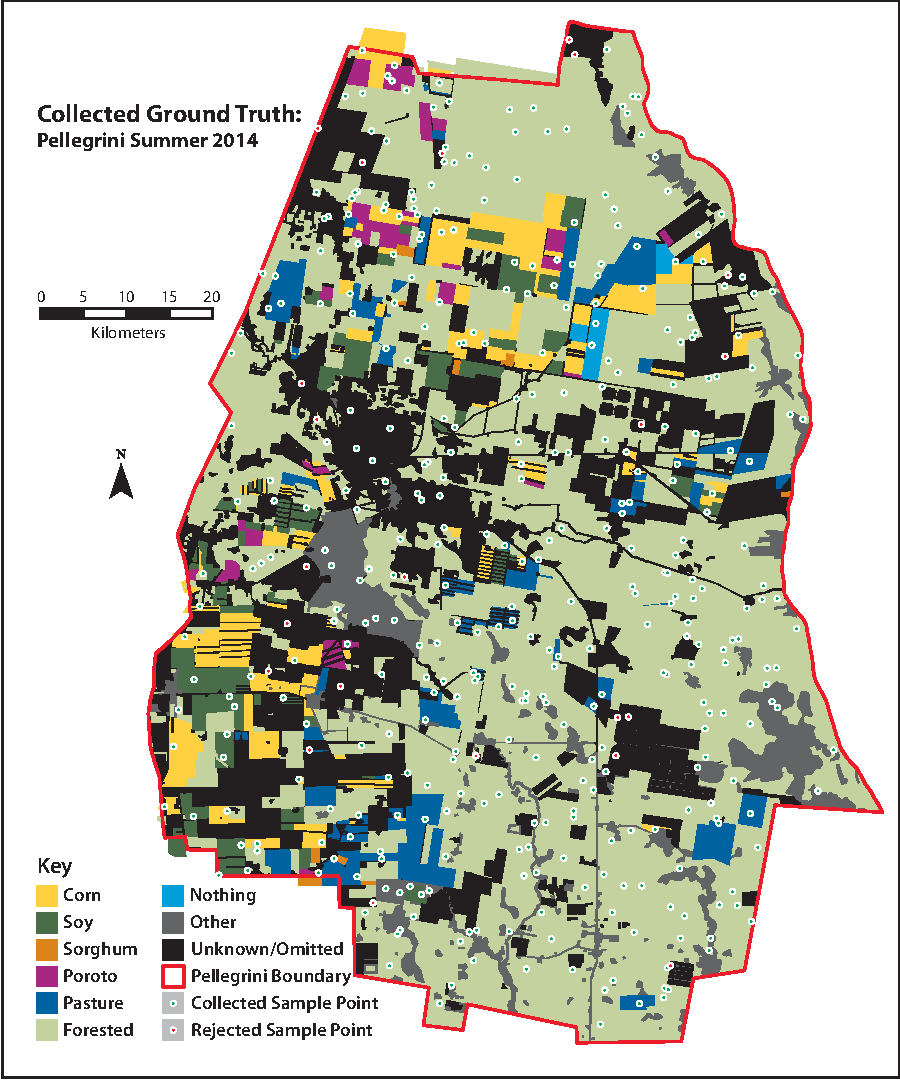
\includegraphics[width=\textwidth]{Graphics/collecteddata.pdf}
  \caption{Pellegrini Summer 2014 Collected and Digitized Ground Truth Dataset}
  \label{map:pellegrini:groundtruth}
\end{ssfigure}
Of my 400 sample points, I was able to visually classify 247 of the points as forested from Landsat OLI imagery before leaving for Argentina. Of the remaining 153, I identified 106 as actively-cultivated agriculture: thirty six points as corn, twenty four points as soy, two points as sorghum, seven points as poroto, and thirty seven points as pasture. Twenty two points were identified as ``other,'' representing all non-forest, non-agricultural, and/or mixed-use land cover classes. Another three points, based on the literal descriptions communicated to me by land managers, were identified as ``nothing.'' I am unsure if these fields were simply left fallow or are something else, but they are not under active cultivation. Twenty two points could not be verified due to inaccessibility, uncertainty, or falling on a mixed-use area, and were removed from the final set of sample points used for the accuracy assessment.

I tried to get direct observations of all crop sample points to accurately record the crop types. However, this strategy proved to be difficult in many cases; I was able to visit only forty seven of the crop points. Often, fields were inaccessible due to road conditions or locked gated. Forty five crop observations came from interviews with farmers and land owners. In a few cases I was able to meet with agricultural engineers who were even able to provide me with maps of the fields they managed (see \autoref{pic:localmap}).
\begin{ssfigure}
  \centering
  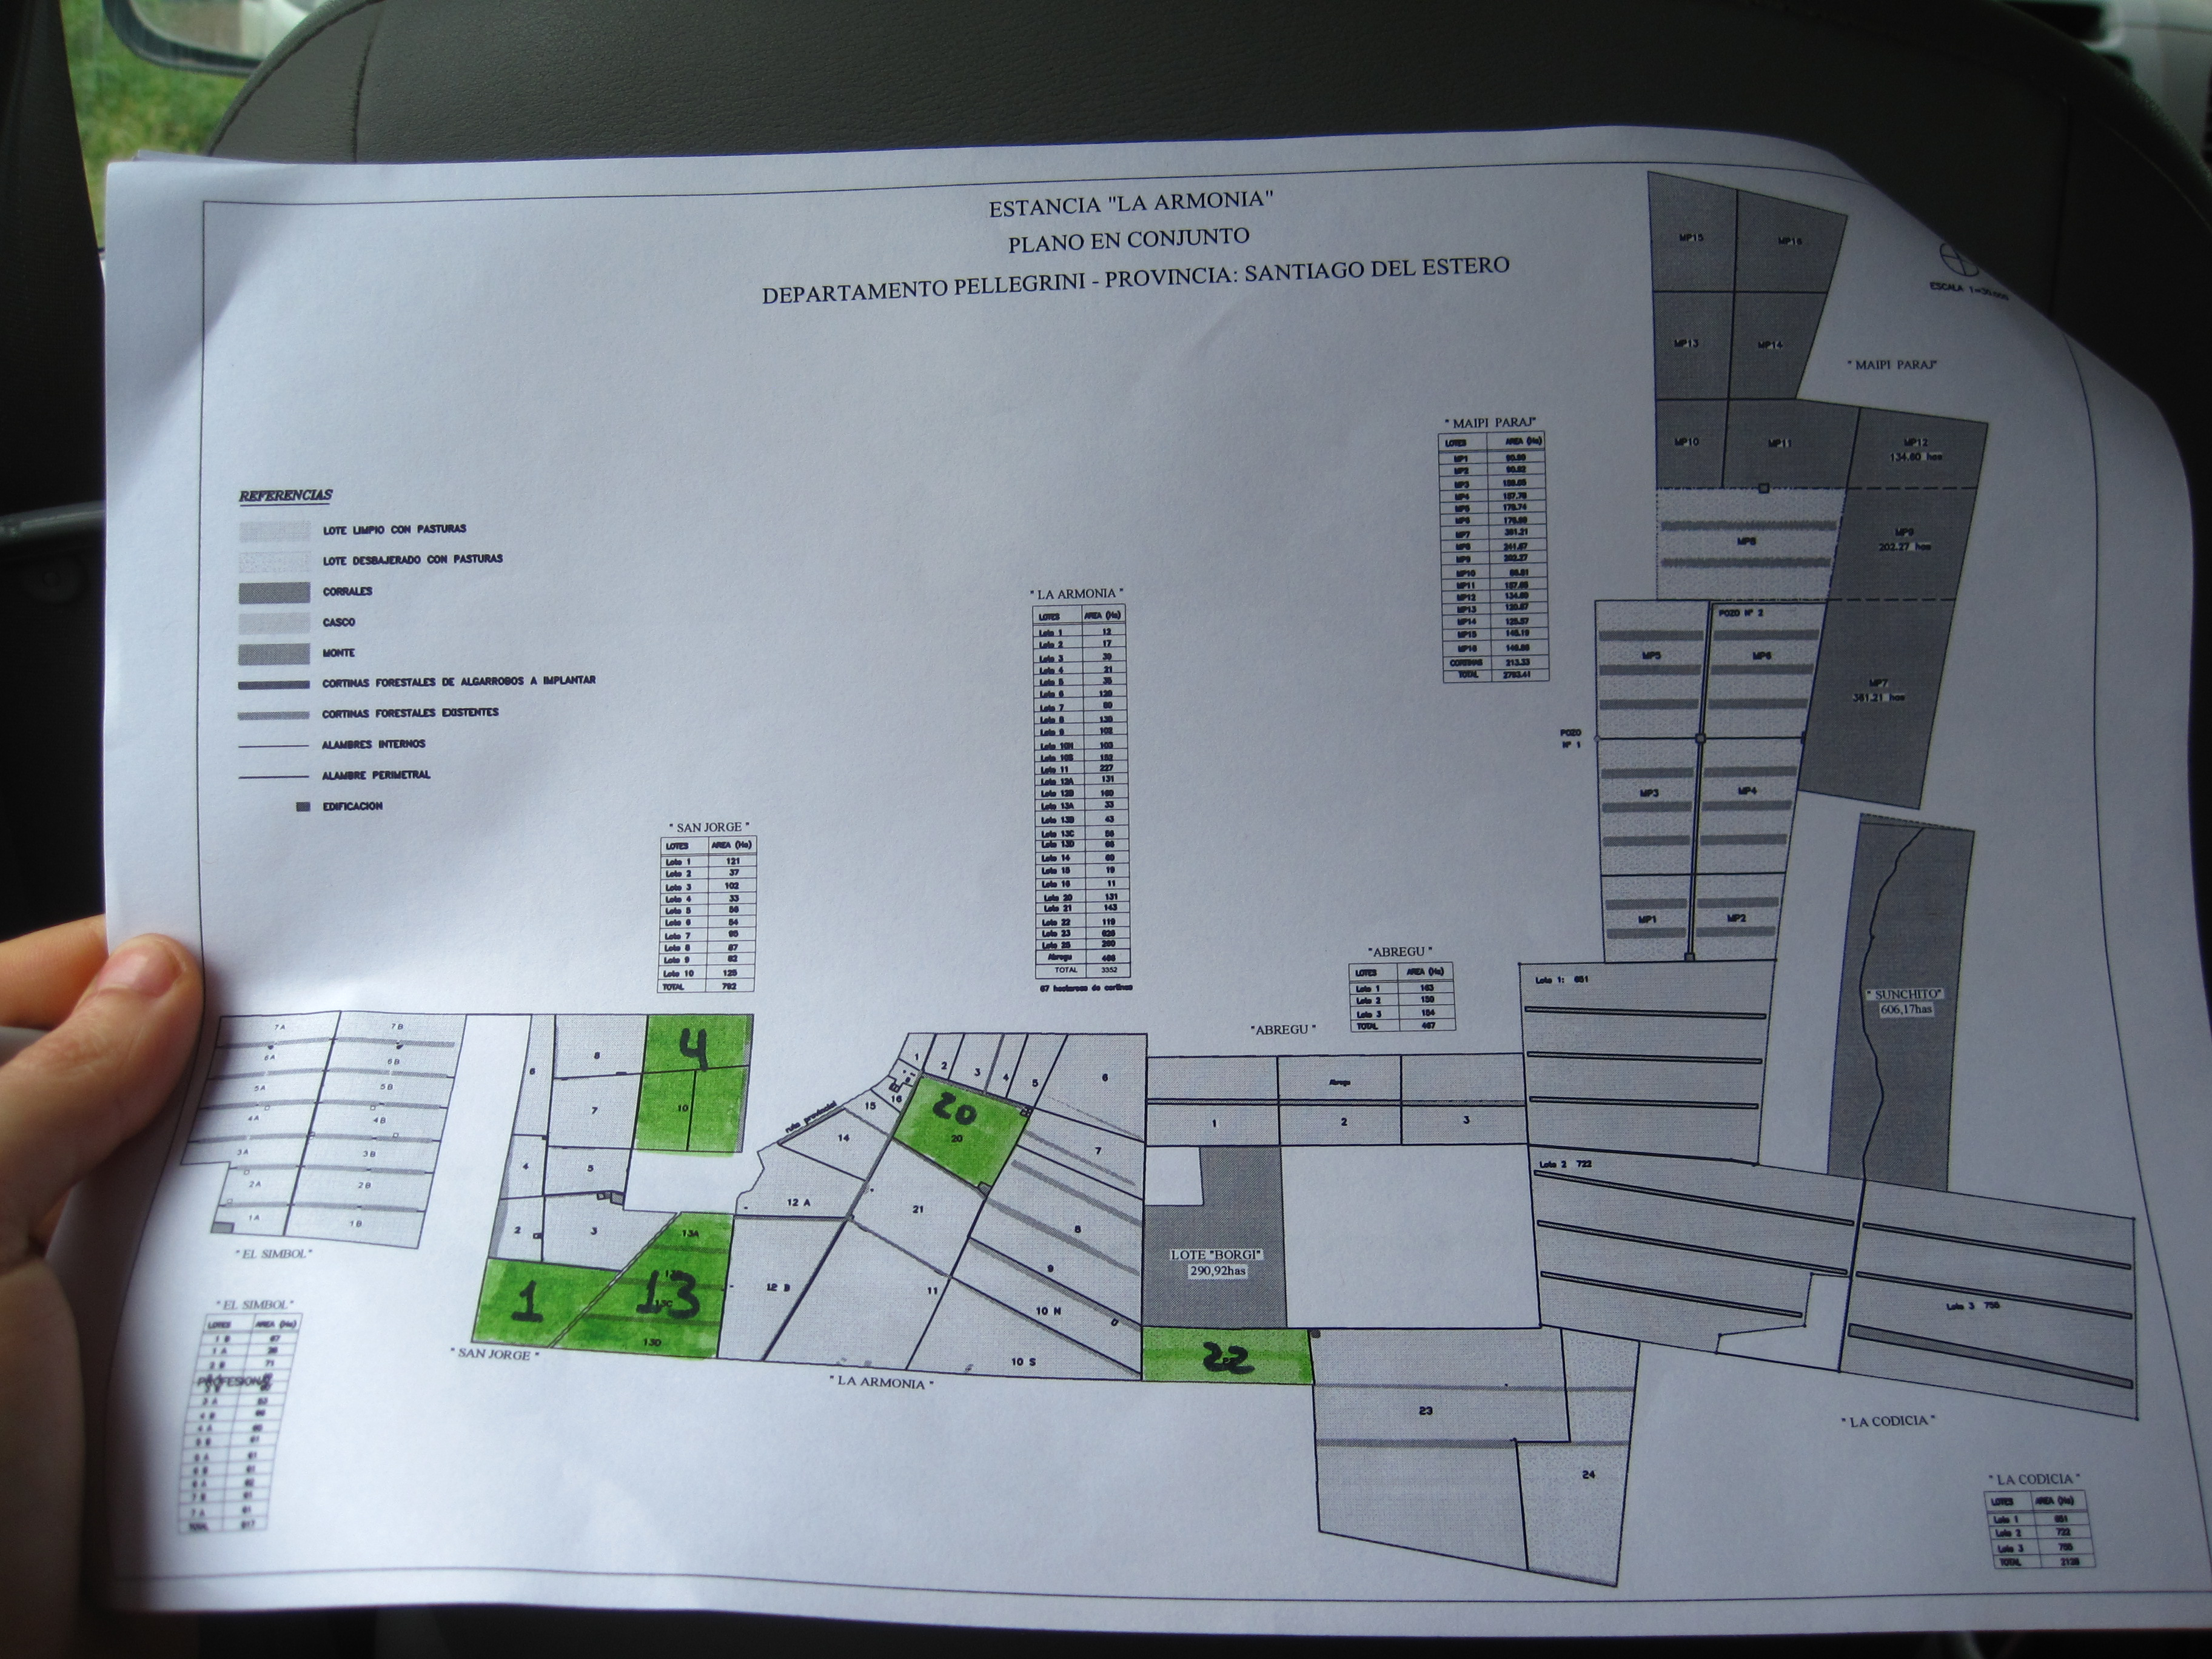
\includegraphics[width=1.0\textwidth]{Graphics/Pics/map.png}
  \caption{Map of \textit{Estancia La Armonia}, a Large Farm}
  \label{pic:localmap}
  \medskip
  \small
  This map is exemplary of those used by the larger farming operations to plan their land use. This farm, \textit{Estancia La Armonia}, primarily raises cattle, so most all of the fields shown are pasture areas. The fields shown highlighted in green are sorghum, which I was told is used as part of the feed mixture in a small cattle feedlot operation.
\end{ssfigure}
The last fourteen crop point identifications were interpreted from Landsat imagery.

The total area of each of land cover class is shown in \autoref{table:pellegrini:LCarea}.
\begin{sstable}
  \centering
  \caption[Summer 2014 Pellegrini Land Cover Classes, From Ground Truth]{Summer 2014 Pellegrini Land Cover Classes, From Ground Truth\\~By Area, with Sample Point Counts}
  \label{table:pellegrini:LCarea}
  \begin{tabu}{XX[r]X[r]}
    \toprule
    \textbf{Cover Type} & \textbf{Hectares} & \textbf{Sample Points} \\
    \midrule
    Forested & 389,541 & 247 \\
    Other & 42,229 & 22 \\
    Corn & 41,488 & 36 \\
    Pasture & 35,057 & 37 \\
    Soy & 27,498 & 24 \\
    Poroto & 9,539 & 7 \\
    Nothing & 3,057 & 3 \\
    Sorghum & 1,646 & 2 \\
    \midrule
    Unknown & 92,248 & 17 \\
    Omitted & 52,052 & 5 \\
    \midrule
    \textbf{Total} & 694,346 & 400 \\
    \bottomrule
  \end{tabu}
\end{sstable}
Compared to the 2000 through 2005 crop areas from \textcite{volante2005analisis}, corn seems to have expanded significantly in the area, while soy has retreated, despite the impression of the contrary in the country as a whole. I gathered from talks with farmers that the decline of soy may be due to increased expenses in the region due to pests, fungus, poor soil, and transportation. Sorghum, a hectare count of which \citeauthor{volante2005analisis} omitted for Pellegrini, does not occupy much land relative to the other crops, and, across Argentina as a whole, experienced a significant decline in production from 1970 to 2003 \autocite{paruelo2005expansion}. However, the 1,646 hectares I observed may indicate a reversal of sorghum's popularity due to increasing demand as cattle feed in feedlots, and could likely be a bigger piece of the Pellegrini agricultural pie in coming years.

In conferring with local farmers and land owners, I found the typical planting and harvesting dates for the major summer crops of soy, corn, sorghum, and poroto, shown in \autoref{table:plantingdates}.
\begin{sstable}
  \centering
  \caption{Typical Planting Dates for Summer Crops, Pellegrini, Argentina}
  \label{table:plantingdates}
  \begin{tabu}{X[0.45,m,c]X[1,m,c]X[.95,m,c]X[0.5,m,c]}
    \toprule
    \textbf{Crop} & \textbf{Ideal Planting Range} & \textbf{Latest Planting Date} & \textbf{Harvesting Begins} \\
    \midrule
    Soy & \datenoyear{15}{12} to \datenoyear{15}{1} & End of February & \datenoyear{1}{5} \\
    Corn & \datenoyear{15}{1} to \datenoyear{15}{2} & End of February & \datenoyear{1}{6} \\
    Sorghum & \datenoyear{15}{1} to \datenoyear{15}{2} & End of February & \datenoyear{1}{6} \\
    Poroto & \datenoyear{15}{1} to \datenoyear{20}{2} & Early March & \datenoyear{10}{5} \\
    \bottomrule
  \end{tabu}
\end{sstable}
The dates I collected did not match those I found published for the country as a whole (see \autoref{studyareas:pellegrini}, \autopageref{studyareas:pellegrini}). In fact, based on my data, soy is most frequently planted before corn, in contrast to Kansas and the rest of Argentina (see \autoref{table:KSplantingdates} on \autopageref{table:KSplantingdates} for Kansas dates). I was also told that the winter growing season is separate from the summer growing season. Unlike Kansas, where the beginning of the summer crops (namely corn's early development) overlaps with the end of winter wheat growth, the harvesting of Pellegrini's winter crops is typically completed before summer planting begins. Thus, where double cropping is limited in Kansas to a winter crop and a late-developing summer crop (overwhelmingly a winter wheat and soy or winter wheat and sorghum combination), any winter crop can be paired with any summer crop in Pellegrini.


\section{Elimination of Mixels}

I found 1,359 pure pixels in the 100 pixel by 100 pixel Kansas study area. The low percentage of pure pixels in the study area is due to the large pixel size relative to the fields, as well as a few irregular features cutting across the pixel grid. The distribution of pure pixels across the land classes is shown in \autoref{table:mixels}.

%\todo[inline]{FIGURE OUT HOW TO USE S COLUMN FROM SIUNITX TO ALIGN NUMBERS ON DECIMAL POINT WHILE USING CENTERING FOR COLUMNS}
%
%\begin{sstable}
%  \centering
%  \caption{Mixel and Pure Pixel Counts}
%  \label{table:mixels}
%  \begin{tabu}{X[1]|X[0.6,r]X[1,r]|X[0.6,r]X[1,r]}
%    \toprule
%     & \multicolumn{2}{c|}{\textbf{Summer 2012 Kansas TSI}} & \multicolumn{2}{c}{\textbf{Summer 2014 Pellegrini TSI}} \\
%    & Count & Percent of Total & Count & Percent of Total \\
%    \midrule
%    \textbf{Total Pixels} & 10,000 & 100.00 & 129,873 & 100.00 \\
%    \ \ \ \ Pure Pixels & 1,359 & 13.59 & 97,054 & 74.73 \\
%    \ \ \ \ \ \ \ \ Corn & 414 & 4.14 & 5,855 & 4.51 \\
%    \ \ \ \ \ \ \ \ Soy & 354 & 3.54 & 3,936 & 3.03 \\
%    \ \ \ \ \ \ \ \ Sorghum & 16 & 0.16 & 183 & 0.14 \\
%    \ \ \ \ \ \ \ \ Unknown & --- & --- & 10,676 & 8.22 \\
%    \ \ \ \ \ \ \ \ All Others & 575 & 5.75 & 76,404 & 58.83 \\
%    \ \ \ \ Mixels & 8,641 & 86.41 & 32,819 & 25.27 \\
%    \bottomrule
%  \end{tabu}
%\end{sstable}

\begin{sstable}
  \centering
  \caption{Summer 2012 Kansas TSI Mixel and Pure Pixel Counts}
  \label{table:mixels}
  \begin{tabu} to 4in {XX[r]X[r]}
    \toprule
     & Count & Percent of Total \\
    \midrule
    \textbf{Total Pixels} & 10,000 & 100.00 \\
    \ \ \ \ Pure Pixels & 1,359 & 13.59 \\
    \ \ \ \ \ \ \ \ \textit{Corn} & 414 & 4.14 \\
    \ \ \ \ \ \ \ \ \textit{Soy} & 354 & 3.54 \\
    \ \ \ \ \ \ \ \ \textit{Sorghum} & 16 & 0.16 \\
    \ \ \ \ \ \ \ \ \textit{All Others} & 575 & 5.75 \\
    \ \ \ \ Mixels & 8,641 & 86.41 \\
    \bottomrule
  \end{tabu}
\end{sstable}


\section{Extracted Reference Signatures}

Before extracting the reference signatures for each summer crop, the pixels for each crop had to be clustered. \autoref{map:KSclusters} shows the spatial distribution of the three clusters for each crop. Given the small number of pixels, the k-means algorithm only found a single cluster for sorghum.

\begin{ssfigure}
  \centering
  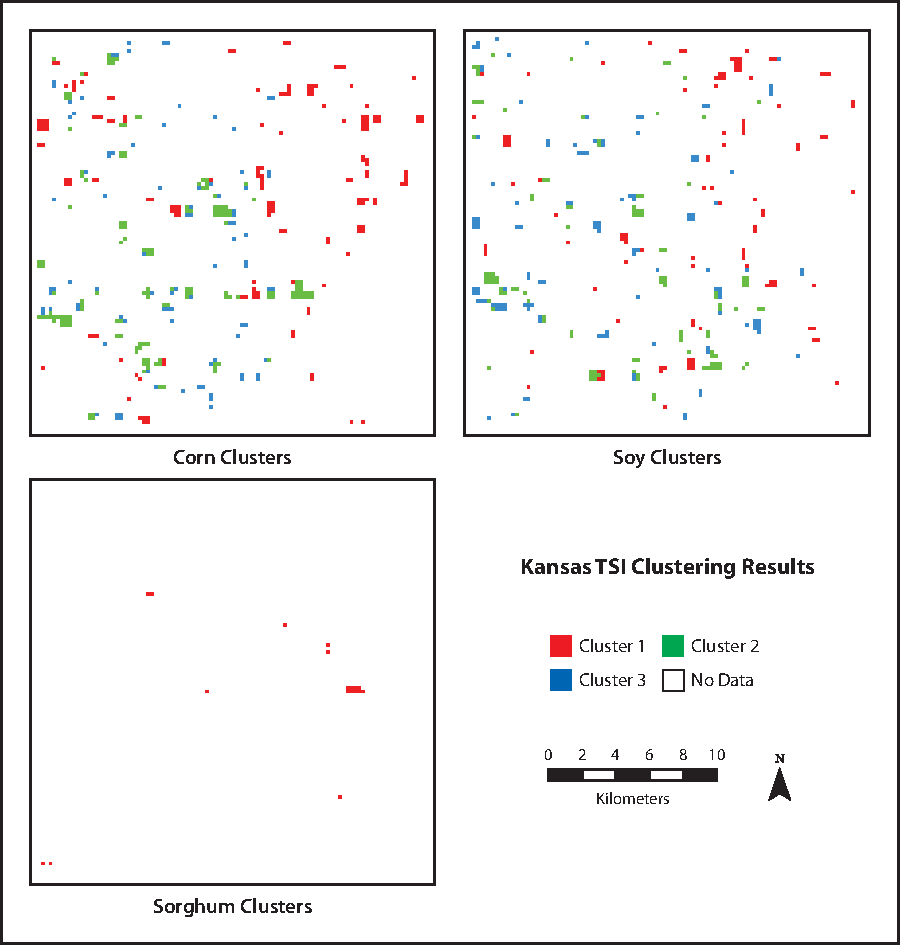
\includegraphics[width=\textwidth]{Graphics/KSclustered.pdf}
  \caption{Clustering the Kansas TSI Image into Three Clusters for Each Crop}
  \label{map:KSclusters}
\end{ssfigure}

The temporal signatures of each of the clusters are plotted in \autoref{fig:KScropsigs}. Each of the crops have a somewhat similar appearance to one another, but each can be differentiated: corn peaks earlier in the year than soy or sorghum, soy has a rounder peak than corn, while sorghum has lower VI values and a slightly later growing season than soy.

\begin{ssfigure}
  \centering
  %%Signature of ['Soy', 'Corn', 'Sorghum'] from /Users/phoetrymaster/Documents/School/Geography/Thesis/Data/MODIS_KANSAS_2007-2012/reprojected/Summer2012/kmeansTesting_2/KMEANS2_SIGS/ processed with allsigsKS.py.
%% Creator: Matplotlib, PGF backend
%%
%% To include the figure in your LaTeX document, write
%%   \input{<filename>.pgf}
%%
%% Make sure the required packages are loaded in your preamble
%%   \usepackage{pgf}
%%
%% Figures using additional raster images can only be included by \input if
%% they are in the same directory as the main LaTeX file. For loading figures
%% from other directories you can use the `import` package
%%   \usepackage{import}
%% and then include the figures with
%%   \import{<path to file>}{<filename>.pgf}
%%
%% Matplotlib used the following preamble
%%   \usepackage{fontspec}
%%   \setsansfont{Myriad Pro}
%%   \setmonofont{Bitstream Vera Sans Mono}
%%
\begingroup%
\makeatletter%
\begin{pgfpicture}%
\pgfpathrectangle{\pgfpointorigin}{\pgfqpoint{5.149972in}{5.326875in}}%
\pgfusepath{use as bounding box}%
\begin{pgfscope}%
\pgfsetbuttcap%
\pgfsetroundjoin%
\definecolor{currentfill}{rgb}{1.000000,1.000000,1.000000}%
\pgfsetfillcolor{currentfill}%
\pgfsetlinewidth{0.000000pt}%
\definecolor{currentstroke}{rgb}{1.000000,1.000000,1.000000}%
\pgfsetstrokecolor{currentstroke}%
\pgfsetdash{}{0pt}%
\pgfpathmoveto{\pgfqpoint{-0.000000in}{0.000000in}}%
\pgfpathlineto{\pgfqpoint{5.149972in}{0.000000in}}%
\pgfpathlineto{\pgfqpoint{5.149972in}{5.326875in}}%
\pgfpathlineto{\pgfqpoint{-0.000000in}{5.326875in}}%
\pgfpathclose%
\pgfusepath{fill}%
\end{pgfscope}%
\begin{pgfscope}%
\pgfsetbuttcap%
\pgfsetroundjoin%
\definecolor{currentfill}{rgb}{0.898039,0.898039,0.898039}%
\pgfsetfillcolor{currentfill}%
\pgfsetlinewidth{0.000000pt}%
\definecolor{currentstroke}{rgb}{0.000000,0.000000,0.000000}%
\pgfsetstrokecolor{currentstroke}%
\pgfsetstrokeopacity{0.000000}%
\pgfsetdash{}{0pt}%
\pgfpathmoveto{\pgfqpoint{0.593722in}{1.226875in}}%
\pgfpathlineto{\pgfqpoint{5.049972in}{1.226875in}}%
\pgfpathlineto{\pgfqpoint{5.049972in}{5.226875in}}%
\pgfpathlineto{\pgfqpoint{0.593722in}{5.226875in}}%
\pgfpathclose%
\pgfusepath{fill}%
\end{pgfscope}%
\begin{pgfscope}%
\pgfpathrectangle{\pgfqpoint{0.593722in}{1.226875in}}{\pgfqpoint{4.456250in}{4.000000in}} %
\pgfusepath{clip}%
\pgfsetroundcap%
\pgfsetroundjoin%
\pgfsetlinewidth{1.003750pt}%
\definecolor{currentstroke}{rgb}{1.000000,1.000000,1.000000}%
\pgfsetstrokecolor{currentstroke}%
\pgfsetdash{}{0pt}%
\pgfpathmoveto{\pgfqpoint{0.936511in}{1.226875in}}%
\pgfpathlineto{\pgfqpoint{0.936511in}{5.226875in}}%
\pgfusepath{stroke}%
\end{pgfscope}%
\begin{pgfscope}%
\pgfsetbuttcap%
\pgfsetroundjoin%
\definecolor{currentfill}{rgb}{0.5,0.5,0.5}%
\pgfsetfillcolor{currentfill}%
\pgfsetlinewidth{1.003750pt}%
\definecolor{currentstroke}{rgb}{0.5,0.5,0.5}%
\pgfsetstrokecolor{currentstroke}%
\pgfsetdash{}{0pt}%
\pgfsys@defobject{currentmarker}{\pgfqpoint{0.000000in}{-0.055556in}}{\pgfqpoint{0.000000in}{0.000000in}}{%
\pgfpathmoveto{\pgfqpoint{0.000000in}{0.000000in}}%
\pgfpathlineto{\pgfqpoint{0.000000in}{-0.055556in}}%
\pgfusepath{stroke,fill}%
}%
\begin{pgfscope}%
\pgfsys@transformshift{0.936511in}{1.226875in}%
\pgfsys@useobject{currentmarker}{}%
\end{pgfscope}%
\end{pgfscope}%
\begin{pgfscope}%
\definecolor{textcolor}{rgb}{0.5,0.5,0.5}%
\pgfsetstrokecolor{textcolor}%
\pgfsetfillcolor{textcolor}%
\pgftext[x=0.936511in,y=1.115763in,,top]{{\rmfamily\fontsize{10.000000}{12.000000}\selectfont\color{textcolor} 97}}%
\end{pgfscope}%
\begin{pgfscope}%
\pgfpathrectangle{\pgfqpoint{0.593722in}{1.226875in}}{\pgfqpoint{4.456250in}{4.000000in}} %
\pgfusepath{clip}%
\pgfsetroundcap%
\pgfsetroundjoin%
\pgfsetlinewidth{1.003750pt}%
\definecolor{currentstroke}{rgb}{1.000000,1.000000,1.000000}%
\pgfsetstrokecolor{currentstroke}%
\pgfsetdash{}{0pt}%
\pgfpathmoveto{\pgfqpoint{1.622087in}{1.226875in}}%
\pgfpathlineto{\pgfqpoint{1.622087in}{5.226875in}}%
\pgfusepath{stroke}%
\end{pgfscope}%
\begin{pgfscope}%
\pgfsetbuttcap%
\pgfsetroundjoin%
\definecolor{currentfill}{rgb}{0.5,0.5,0.5}%
\pgfsetfillcolor{currentfill}%
\pgfsetlinewidth{1.003750pt}%
\definecolor{currentstroke}{rgb}{0.5,0.5,0.5}%
\pgfsetstrokecolor{currentstroke}%
\pgfsetdash{}{0pt}%
\pgfsys@defobject{currentmarker}{\pgfqpoint{0.000000in}{-0.055556in}}{\pgfqpoint{0.000000in}{0.000000in}}{%
\pgfpathmoveto{\pgfqpoint{0.000000in}{0.000000in}}%
\pgfpathlineto{\pgfqpoint{0.000000in}{-0.055556in}}%
\pgfusepath{stroke,fill}%
}%
\begin{pgfscope}%
\pgfsys@transformshift{1.622087in}{1.226875in}%
\pgfsys@useobject{currentmarker}{}%
\end{pgfscope}%
\end{pgfscope}%
\begin{pgfscope}%
\definecolor{textcolor}{rgb}{0.5,0.5,0.5}%
\pgfsetstrokecolor{textcolor}%
\pgfsetfillcolor{textcolor}%
\pgftext[x=1.622087in,y=1.115763in,,top]{{\rmfamily\fontsize{10.000000}{12.000000}\selectfont\color{textcolor} 129}}%
\end{pgfscope}%
\begin{pgfscope}%
\pgfpathrectangle{\pgfqpoint{0.593722in}{1.226875in}}{\pgfqpoint{4.456250in}{4.000000in}} %
\pgfusepath{clip}%
\pgfsetroundcap%
\pgfsetroundjoin%
\pgfsetlinewidth{1.003750pt}%
\definecolor{currentstroke}{rgb}{1.000000,1.000000,1.000000}%
\pgfsetstrokecolor{currentstroke}%
\pgfsetdash{}{0pt}%
\pgfpathmoveto{\pgfqpoint{2.307664in}{1.226875in}}%
\pgfpathlineto{\pgfqpoint{2.307664in}{5.226875in}}%
\pgfusepath{stroke}%
\end{pgfscope}%
\begin{pgfscope}%
\pgfsetbuttcap%
\pgfsetroundjoin%
\definecolor{currentfill}{rgb}{0.5,0.5,0.5}%
\pgfsetfillcolor{currentfill}%
\pgfsetlinewidth{1.003750pt}%
\definecolor{currentstroke}{rgb}{0.5,0.5,0.5}%
\pgfsetstrokecolor{currentstroke}%
\pgfsetdash{}{0pt}%
\pgfsys@defobject{currentmarker}{\pgfqpoint{0.000000in}{-0.055556in}}{\pgfqpoint{0.000000in}{0.000000in}}{%
\pgfpathmoveto{\pgfqpoint{0.000000in}{0.000000in}}%
\pgfpathlineto{\pgfqpoint{0.000000in}{-0.055556in}}%
\pgfusepath{stroke,fill}%
}%
\begin{pgfscope}%
\pgfsys@transformshift{2.307664in}{1.226875in}%
\pgfsys@useobject{currentmarker}{}%
\end{pgfscope}%
\end{pgfscope}%
\begin{pgfscope}%
\definecolor{textcolor}{rgb}{0.5,0.5,0.5}%
\pgfsetstrokecolor{textcolor}%
\pgfsetfillcolor{textcolor}%
\pgftext[x=2.307664in,y=1.115763in,,top]{{\rmfamily\fontsize{10.000000}{12.000000}\selectfont\color{textcolor} 161}}%
\end{pgfscope}%
\begin{pgfscope}%
\pgfpathrectangle{\pgfqpoint{0.593722in}{1.226875in}}{\pgfqpoint{4.456250in}{4.000000in}} %
\pgfusepath{clip}%
\pgfsetroundcap%
\pgfsetroundjoin%
\pgfsetlinewidth{1.003750pt}%
\definecolor{currentstroke}{rgb}{1.000000,1.000000,1.000000}%
\pgfsetstrokecolor{currentstroke}%
\pgfsetdash{}{0pt}%
\pgfpathmoveto{\pgfqpoint{2.993241in}{1.226875in}}%
\pgfpathlineto{\pgfqpoint{2.993241in}{5.226875in}}%
\pgfusepath{stroke}%
\end{pgfscope}%
\begin{pgfscope}%
\pgfsetbuttcap%
\pgfsetroundjoin%
\definecolor{currentfill}{rgb}{0.5,0.5,0.5}%
\pgfsetfillcolor{currentfill}%
\pgfsetlinewidth{1.003750pt}%
\definecolor{currentstroke}{rgb}{0.5,0.5,0.5}%
\pgfsetstrokecolor{currentstroke}%
\pgfsetdash{}{0pt}%
\pgfsys@defobject{currentmarker}{\pgfqpoint{0.000000in}{-0.055556in}}{\pgfqpoint{0.000000in}{0.000000in}}{%
\pgfpathmoveto{\pgfqpoint{0.000000in}{0.000000in}}%
\pgfpathlineto{\pgfqpoint{0.000000in}{-0.055556in}}%
\pgfusepath{stroke,fill}%
}%
\begin{pgfscope}%
\pgfsys@transformshift{2.993241in}{1.226875in}%
\pgfsys@useobject{currentmarker}{}%
\end{pgfscope}%
\end{pgfscope}%
\begin{pgfscope}%
\definecolor{textcolor}{rgb}{0.5,0.5,0.5}%
\pgfsetstrokecolor{textcolor}%
\pgfsetfillcolor{textcolor}%
\pgftext[x=2.993241in,y=1.115763in,,top]{{\rmfamily\fontsize{10.000000}{12.000000}\selectfont\color{textcolor} 193}}%
\end{pgfscope}%
\begin{pgfscope}%
\pgfpathrectangle{\pgfqpoint{0.593722in}{1.226875in}}{\pgfqpoint{4.456250in}{4.000000in}} %
\pgfusepath{clip}%
\pgfsetroundcap%
\pgfsetroundjoin%
\pgfsetlinewidth{1.003750pt}%
\definecolor{currentstroke}{rgb}{1.000000,1.000000,1.000000}%
\pgfsetstrokecolor{currentstroke}%
\pgfsetdash{}{0pt}%
\pgfpathmoveto{\pgfqpoint{3.678818in}{1.226875in}}%
\pgfpathlineto{\pgfqpoint{3.678818in}{5.226875in}}%
\pgfusepath{stroke}%
\end{pgfscope}%
\begin{pgfscope}%
\pgfsetbuttcap%
\pgfsetroundjoin%
\definecolor{currentfill}{rgb}{0.5,0.5,0.5}%
\pgfsetfillcolor{currentfill}%
\pgfsetlinewidth{1.003750pt}%
\definecolor{currentstroke}{rgb}{0.5,0.5,0.5}%
\pgfsetstrokecolor{currentstroke}%
\pgfsetdash{}{0pt}%
\pgfsys@defobject{currentmarker}{\pgfqpoint{0.000000in}{-0.055556in}}{\pgfqpoint{0.000000in}{0.000000in}}{%
\pgfpathmoveto{\pgfqpoint{0.000000in}{0.000000in}}%
\pgfpathlineto{\pgfqpoint{0.000000in}{-0.055556in}}%
\pgfusepath{stroke,fill}%
}%
\begin{pgfscope}%
\pgfsys@transformshift{3.678818in}{1.226875in}%
\pgfsys@useobject{currentmarker}{}%
\end{pgfscope}%
\end{pgfscope}%
\begin{pgfscope}%
\definecolor{textcolor}{rgb}{0.5,0.5,0.5}%
\pgfsetstrokecolor{textcolor}%
\pgfsetfillcolor{textcolor}%
\pgftext[x=3.678818in,y=1.115763in,,top]{{\rmfamily\fontsize{10.000000}{12.000000}\selectfont\color{textcolor} 225}}%
\end{pgfscope}%
\begin{pgfscope}%
\pgfpathrectangle{\pgfqpoint{0.593722in}{1.226875in}}{\pgfqpoint{4.456250in}{4.000000in}} %
\pgfusepath{clip}%
\pgfsetroundcap%
\pgfsetroundjoin%
\pgfsetlinewidth{1.003750pt}%
\definecolor{currentstroke}{rgb}{1.000000,1.000000,1.000000}%
\pgfsetstrokecolor{currentstroke}%
\pgfsetdash{}{0pt}%
\pgfpathmoveto{\pgfqpoint{4.364395in}{1.226875in}}%
\pgfpathlineto{\pgfqpoint{4.364395in}{5.226875in}}%
\pgfusepath{stroke}%
\end{pgfscope}%
\begin{pgfscope}%
\pgfsetbuttcap%
\pgfsetroundjoin%
\definecolor{currentfill}{rgb}{0.5,0.5,0.5}%
\pgfsetfillcolor{currentfill}%
\pgfsetlinewidth{1.003750pt}%
\definecolor{currentstroke}{rgb}{0.5,0.5,0.5}%
\pgfsetstrokecolor{currentstroke}%
\pgfsetdash{}{0pt}%
\pgfsys@defobject{currentmarker}{\pgfqpoint{0.000000in}{-0.055556in}}{\pgfqpoint{0.000000in}{0.000000in}}{%
\pgfpathmoveto{\pgfqpoint{0.000000in}{0.000000in}}%
\pgfpathlineto{\pgfqpoint{0.000000in}{-0.055556in}}%
\pgfusepath{stroke,fill}%
}%
\begin{pgfscope}%
\pgfsys@transformshift{4.364395in}{1.226875in}%
\pgfsys@useobject{currentmarker}{}%
\end{pgfscope}%
\end{pgfscope}%
\begin{pgfscope}%
\definecolor{textcolor}{rgb}{0.5,0.5,0.5}%
\pgfsetstrokecolor{textcolor}%
\pgfsetfillcolor{textcolor}%
\pgftext[x=4.364395in,y=1.115763in,,top]{{\rmfamily\fontsize{10.000000}{12.000000}\selectfont\color{textcolor} 257}}%
\end{pgfscope}%
\begin{pgfscope}%
\pgfpathrectangle{\pgfqpoint{0.593722in}{1.226875in}}{\pgfqpoint{4.456250in}{4.000000in}} %
\pgfusepath{clip}%
\pgfsetroundcap%
\pgfsetroundjoin%
\pgfsetlinewidth{0.501875pt}%
\definecolor{currentstroke}{rgb}{1.000000,1.000000,1.000000}%
\pgfsetstrokecolor{currentstroke}%
\pgfsetdash{}{0pt}%
\pgfpathmoveto{\pgfqpoint{0.936511in}{1.226875in}}%
\pgfpathlineto{\pgfqpoint{0.936511in}{5.226875in}}%
\pgfusepath{stroke}%
\end{pgfscope}%
\begin{pgfscope}%
\pgfsetbuttcap%
\pgfsetroundjoin%
\definecolor{currentfill}{rgb}{0.5,0.5,0.5}%
\pgfsetfillcolor{currentfill}%
\pgfsetlinewidth{0.501875pt}%
\definecolor{currentstroke}{rgb}{0.5,0.5,0.5}%
\pgfsetstrokecolor{currentstroke}%
\pgfsetdash{}{0pt}%
\pgfsys@defobject{currentmarker}{\pgfqpoint{0.000000in}{0.000000in}}{\pgfqpoint{0.000000in}{0.000000in}}{%
\pgfpathmoveto{\pgfqpoint{0.000000in}{0.000000in}}%
\pgfpathlineto{\pgfqpoint{0.000000in}{0.000000in}}%
\pgfusepath{stroke,fill}%
}%
\begin{pgfscope}%
\pgfsys@transformshift{0.936511in}{1.226875in}%
\pgfsys@useobject{currentmarker}{}%
\end{pgfscope}%
\end{pgfscope}%
\begin{pgfscope}%
\pgfsetbuttcap%
\pgfsetroundjoin%
\definecolor{currentfill}{rgb}{0.5,0.5,0.5}%
\pgfsetfillcolor{currentfill}%
\pgfsetlinewidth{0.501875pt}%
\definecolor{currentstroke}{rgb}{0.5,0.5,0.5}%
\pgfsetstrokecolor{currentstroke}%
\pgfsetdash{}{0pt}%
\pgfsys@defobject{currentmarker}{\pgfqpoint{0.000000in}{0.000000in}}{\pgfqpoint{0.000000in}{0.000000in}}{%
\pgfpathmoveto{\pgfqpoint{0.000000in}{0.000000in}}%
\pgfpathlineto{\pgfqpoint{0.000000in}{0.000000in}}%
\pgfusepath{stroke,fill}%
}%
\begin{pgfscope}%
\pgfsys@transformshift{0.936511in}{5.226875in}%
\pgfsys@useobject{currentmarker}{}%
\end{pgfscope}%
\end{pgfscope}%
\begin{pgfscope}%
\pgfpathrectangle{\pgfqpoint{0.593722in}{1.226875in}}{\pgfqpoint{4.456250in}{4.000000in}} %
\pgfusepath{clip}%
\pgfsetroundcap%
\pgfsetroundjoin%
\pgfsetlinewidth{0.501875pt}%
\definecolor{currentstroke}{rgb}{1.000000,1.000000,1.000000}%
\pgfsetstrokecolor{currentstroke}%
\pgfsetdash{}{0pt}%
\pgfpathmoveto{\pgfqpoint{1.279299in}{1.226875in}}%
\pgfpathlineto{\pgfqpoint{1.279299in}{5.226875in}}%
\pgfusepath{stroke}%
\end{pgfscope}%
\begin{pgfscope}%
\pgfsetbuttcap%
\pgfsetroundjoin%
\definecolor{currentfill}{rgb}{0.5,0.5,0.5}%
\pgfsetfillcolor{currentfill}%
\pgfsetlinewidth{0.501875pt}%
\definecolor{currentstroke}{rgb}{0.5,0.5,0.5}%
\pgfsetstrokecolor{currentstroke}%
\pgfsetdash{}{0pt}%
\pgfsys@defobject{currentmarker}{\pgfqpoint{0.000000in}{0.000000in}}{\pgfqpoint{0.000000in}{0.000000in}}{%
\pgfpathmoveto{\pgfqpoint{0.000000in}{0.000000in}}%
\pgfpathlineto{\pgfqpoint{0.000000in}{0.000000in}}%
\pgfusepath{stroke,fill}%
}%
\begin{pgfscope}%
\pgfsys@transformshift{1.279299in}{1.226875in}%
\pgfsys@useobject{currentmarker}{}%
\end{pgfscope}%
\end{pgfscope}%
\begin{pgfscope}%
\pgfsetbuttcap%
\pgfsetroundjoin%
\definecolor{currentfill}{rgb}{0.5,0.5,0.5}%
\pgfsetfillcolor{currentfill}%
\pgfsetlinewidth{0.501875pt}%
\definecolor{currentstroke}{rgb}{0.5,0.5,0.5}%
\pgfsetstrokecolor{currentstroke}%
\pgfsetdash{}{0pt}%
\pgfsys@defobject{currentmarker}{\pgfqpoint{0.000000in}{0.000000in}}{\pgfqpoint{0.000000in}{0.000000in}}{%
\pgfpathmoveto{\pgfqpoint{0.000000in}{0.000000in}}%
\pgfpathlineto{\pgfqpoint{0.000000in}{0.000000in}}%
\pgfusepath{stroke,fill}%
}%
\begin{pgfscope}%
\pgfsys@transformshift{1.279299in}{5.226875in}%
\pgfsys@useobject{currentmarker}{}%
\end{pgfscope}%
\end{pgfscope}%
\begin{pgfscope}%
\pgfpathrectangle{\pgfqpoint{0.593722in}{1.226875in}}{\pgfqpoint{4.456250in}{4.000000in}} %
\pgfusepath{clip}%
\pgfsetroundcap%
\pgfsetroundjoin%
\pgfsetlinewidth{0.501875pt}%
\definecolor{currentstroke}{rgb}{1.000000,1.000000,1.000000}%
\pgfsetstrokecolor{currentstroke}%
\pgfsetdash{}{0pt}%
\pgfpathmoveto{\pgfqpoint{1.622087in}{1.226875in}}%
\pgfpathlineto{\pgfqpoint{1.622087in}{5.226875in}}%
\pgfusepath{stroke}%
\end{pgfscope}%
\begin{pgfscope}%
\pgfsetbuttcap%
\pgfsetroundjoin%
\definecolor{currentfill}{rgb}{0.5,0.5,0.5}%
\pgfsetfillcolor{currentfill}%
\pgfsetlinewidth{0.501875pt}%
\definecolor{currentstroke}{rgb}{0.5,0.5,0.5}%
\pgfsetstrokecolor{currentstroke}%
\pgfsetdash{}{0pt}%
\pgfsys@defobject{currentmarker}{\pgfqpoint{0.000000in}{0.000000in}}{\pgfqpoint{0.000000in}{0.000000in}}{%
\pgfpathmoveto{\pgfqpoint{0.000000in}{0.000000in}}%
\pgfpathlineto{\pgfqpoint{0.000000in}{0.000000in}}%
\pgfusepath{stroke,fill}%
}%
\begin{pgfscope}%
\pgfsys@transformshift{1.622087in}{1.226875in}%
\pgfsys@useobject{currentmarker}{}%
\end{pgfscope}%
\end{pgfscope}%
\begin{pgfscope}%
\pgfsetbuttcap%
\pgfsetroundjoin%
\definecolor{currentfill}{rgb}{0.5,0.5,0.5}%
\pgfsetfillcolor{currentfill}%
\pgfsetlinewidth{0.501875pt}%
\definecolor{currentstroke}{rgb}{0.5,0.5,0.5}%
\pgfsetstrokecolor{currentstroke}%
\pgfsetdash{}{0pt}%
\pgfsys@defobject{currentmarker}{\pgfqpoint{0.000000in}{0.000000in}}{\pgfqpoint{0.000000in}{0.000000in}}{%
\pgfpathmoveto{\pgfqpoint{0.000000in}{0.000000in}}%
\pgfpathlineto{\pgfqpoint{0.000000in}{0.000000in}}%
\pgfusepath{stroke,fill}%
}%
\begin{pgfscope}%
\pgfsys@transformshift{1.622087in}{5.226875in}%
\pgfsys@useobject{currentmarker}{}%
\end{pgfscope}%
\end{pgfscope}%
\begin{pgfscope}%
\pgfpathrectangle{\pgfqpoint{0.593722in}{1.226875in}}{\pgfqpoint{4.456250in}{4.000000in}} %
\pgfusepath{clip}%
\pgfsetroundcap%
\pgfsetroundjoin%
\pgfsetlinewidth{0.501875pt}%
\definecolor{currentstroke}{rgb}{1.000000,1.000000,1.000000}%
\pgfsetstrokecolor{currentstroke}%
\pgfsetdash{}{0pt}%
\pgfpathmoveto{\pgfqpoint{1.964876in}{1.226875in}}%
\pgfpathlineto{\pgfqpoint{1.964876in}{5.226875in}}%
\pgfusepath{stroke}%
\end{pgfscope}%
\begin{pgfscope}%
\pgfsetbuttcap%
\pgfsetroundjoin%
\definecolor{currentfill}{rgb}{0.5,0.5,0.5}%
\pgfsetfillcolor{currentfill}%
\pgfsetlinewidth{0.501875pt}%
\definecolor{currentstroke}{rgb}{0.5,0.5,0.5}%
\pgfsetstrokecolor{currentstroke}%
\pgfsetdash{}{0pt}%
\pgfsys@defobject{currentmarker}{\pgfqpoint{0.000000in}{0.000000in}}{\pgfqpoint{0.000000in}{0.000000in}}{%
\pgfpathmoveto{\pgfqpoint{0.000000in}{0.000000in}}%
\pgfpathlineto{\pgfqpoint{0.000000in}{0.000000in}}%
\pgfusepath{stroke,fill}%
}%
\begin{pgfscope}%
\pgfsys@transformshift{1.964876in}{1.226875in}%
\pgfsys@useobject{currentmarker}{}%
\end{pgfscope}%
\end{pgfscope}%
\begin{pgfscope}%
\pgfsetbuttcap%
\pgfsetroundjoin%
\definecolor{currentfill}{rgb}{0.5,0.5,0.5}%
\pgfsetfillcolor{currentfill}%
\pgfsetlinewidth{0.501875pt}%
\definecolor{currentstroke}{rgb}{0.5,0.5,0.5}%
\pgfsetstrokecolor{currentstroke}%
\pgfsetdash{}{0pt}%
\pgfsys@defobject{currentmarker}{\pgfqpoint{0.000000in}{0.000000in}}{\pgfqpoint{0.000000in}{0.000000in}}{%
\pgfpathmoveto{\pgfqpoint{0.000000in}{0.000000in}}%
\pgfpathlineto{\pgfqpoint{0.000000in}{0.000000in}}%
\pgfusepath{stroke,fill}%
}%
\begin{pgfscope}%
\pgfsys@transformshift{1.964876in}{5.226875in}%
\pgfsys@useobject{currentmarker}{}%
\end{pgfscope}%
\end{pgfscope}%
\begin{pgfscope}%
\pgfpathrectangle{\pgfqpoint{0.593722in}{1.226875in}}{\pgfqpoint{4.456250in}{4.000000in}} %
\pgfusepath{clip}%
\pgfsetroundcap%
\pgfsetroundjoin%
\pgfsetlinewidth{0.501875pt}%
\definecolor{currentstroke}{rgb}{1.000000,1.000000,1.000000}%
\pgfsetstrokecolor{currentstroke}%
\pgfsetdash{}{0pt}%
\pgfpathmoveto{\pgfqpoint{2.307664in}{1.226875in}}%
\pgfpathlineto{\pgfqpoint{2.307664in}{5.226875in}}%
\pgfusepath{stroke}%
\end{pgfscope}%
\begin{pgfscope}%
\pgfsetbuttcap%
\pgfsetroundjoin%
\definecolor{currentfill}{rgb}{0.5,0.5,0.5}%
\pgfsetfillcolor{currentfill}%
\pgfsetlinewidth{0.501875pt}%
\definecolor{currentstroke}{rgb}{0.5,0.5,0.5}%
\pgfsetstrokecolor{currentstroke}%
\pgfsetdash{}{0pt}%
\pgfsys@defobject{currentmarker}{\pgfqpoint{0.000000in}{0.000000in}}{\pgfqpoint{0.000000in}{0.000000in}}{%
\pgfpathmoveto{\pgfqpoint{0.000000in}{0.000000in}}%
\pgfpathlineto{\pgfqpoint{0.000000in}{0.000000in}}%
\pgfusepath{stroke,fill}%
}%
\begin{pgfscope}%
\pgfsys@transformshift{2.307664in}{1.226875in}%
\pgfsys@useobject{currentmarker}{}%
\end{pgfscope}%
\end{pgfscope}%
\begin{pgfscope}%
\pgfsetbuttcap%
\pgfsetroundjoin%
\definecolor{currentfill}{rgb}{0.5,0.5,0.5}%
\pgfsetfillcolor{currentfill}%
\pgfsetlinewidth{0.501875pt}%
\definecolor{currentstroke}{rgb}{0.5,0.5,0.5}%
\pgfsetstrokecolor{currentstroke}%
\pgfsetdash{}{0pt}%
\pgfsys@defobject{currentmarker}{\pgfqpoint{0.000000in}{0.000000in}}{\pgfqpoint{0.000000in}{0.000000in}}{%
\pgfpathmoveto{\pgfqpoint{0.000000in}{0.000000in}}%
\pgfpathlineto{\pgfqpoint{0.000000in}{0.000000in}}%
\pgfusepath{stroke,fill}%
}%
\begin{pgfscope}%
\pgfsys@transformshift{2.307664in}{5.226875in}%
\pgfsys@useobject{currentmarker}{}%
\end{pgfscope}%
\end{pgfscope}%
\begin{pgfscope}%
\pgfpathrectangle{\pgfqpoint{0.593722in}{1.226875in}}{\pgfqpoint{4.456250in}{4.000000in}} %
\pgfusepath{clip}%
\pgfsetroundcap%
\pgfsetroundjoin%
\pgfsetlinewidth{0.501875pt}%
\definecolor{currentstroke}{rgb}{1.000000,1.000000,1.000000}%
\pgfsetstrokecolor{currentstroke}%
\pgfsetdash{}{0pt}%
\pgfpathmoveto{\pgfqpoint{2.650453in}{1.226875in}}%
\pgfpathlineto{\pgfqpoint{2.650453in}{5.226875in}}%
\pgfusepath{stroke}%
\end{pgfscope}%
\begin{pgfscope}%
\pgfsetbuttcap%
\pgfsetroundjoin%
\definecolor{currentfill}{rgb}{0.5,0.5,0.5}%
\pgfsetfillcolor{currentfill}%
\pgfsetlinewidth{0.501875pt}%
\definecolor{currentstroke}{rgb}{0.5,0.5,0.5}%
\pgfsetstrokecolor{currentstroke}%
\pgfsetdash{}{0pt}%
\pgfsys@defobject{currentmarker}{\pgfqpoint{0.000000in}{0.000000in}}{\pgfqpoint{0.000000in}{0.000000in}}{%
\pgfpathmoveto{\pgfqpoint{0.000000in}{0.000000in}}%
\pgfpathlineto{\pgfqpoint{0.000000in}{0.000000in}}%
\pgfusepath{stroke,fill}%
}%
\begin{pgfscope}%
\pgfsys@transformshift{2.650453in}{1.226875in}%
\pgfsys@useobject{currentmarker}{}%
\end{pgfscope}%
\end{pgfscope}%
\begin{pgfscope}%
\pgfsetbuttcap%
\pgfsetroundjoin%
\definecolor{currentfill}{rgb}{0.5,0.5,0.5}%
\pgfsetfillcolor{currentfill}%
\pgfsetlinewidth{0.501875pt}%
\definecolor{currentstroke}{rgb}{0.5,0.5,0.5}%
\pgfsetstrokecolor{currentstroke}%
\pgfsetdash{}{0pt}%
\pgfsys@defobject{currentmarker}{\pgfqpoint{0.000000in}{0.000000in}}{\pgfqpoint{0.000000in}{0.000000in}}{%
\pgfpathmoveto{\pgfqpoint{0.000000in}{0.000000in}}%
\pgfpathlineto{\pgfqpoint{0.000000in}{0.000000in}}%
\pgfusepath{stroke,fill}%
}%
\begin{pgfscope}%
\pgfsys@transformshift{2.650453in}{5.226875in}%
\pgfsys@useobject{currentmarker}{}%
\end{pgfscope}%
\end{pgfscope}%
\begin{pgfscope}%
\pgfpathrectangle{\pgfqpoint{0.593722in}{1.226875in}}{\pgfqpoint{4.456250in}{4.000000in}} %
\pgfusepath{clip}%
\pgfsetroundcap%
\pgfsetroundjoin%
\pgfsetlinewidth{0.501875pt}%
\definecolor{currentstroke}{rgb}{1.000000,1.000000,1.000000}%
\pgfsetstrokecolor{currentstroke}%
\pgfsetdash{}{0pt}%
\pgfpathmoveto{\pgfqpoint{2.993241in}{1.226875in}}%
\pgfpathlineto{\pgfqpoint{2.993241in}{5.226875in}}%
\pgfusepath{stroke}%
\end{pgfscope}%
\begin{pgfscope}%
\pgfsetbuttcap%
\pgfsetroundjoin%
\definecolor{currentfill}{rgb}{0.5,0.5,0.5}%
\pgfsetfillcolor{currentfill}%
\pgfsetlinewidth{0.501875pt}%
\definecolor{currentstroke}{rgb}{0.5,0.5,0.5}%
\pgfsetstrokecolor{currentstroke}%
\pgfsetdash{}{0pt}%
\pgfsys@defobject{currentmarker}{\pgfqpoint{0.000000in}{0.000000in}}{\pgfqpoint{0.000000in}{0.000000in}}{%
\pgfpathmoveto{\pgfqpoint{0.000000in}{0.000000in}}%
\pgfpathlineto{\pgfqpoint{0.000000in}{0.000000in}}%
\pgfusepath{stroke,fill}%
}%
\begin{pgfscope}%
\pgfsys@transformshift{2.993241in}{1.226875in}%
\pgfsys@useobject{currentmarker}{}%
\end{pgfscope}%
\end{pgfscope}%
\begin{pgfscope}%
\pgfsetbuttcap%
\pgfsetroundjoin%
\definecolor{currentfill}{rgb}{0.5,0.5,0.5}%
\pgfsetfillcolor{currentfill}%
\pgfsetlinewidth{0.501875pt}%
\definecolor{currentstroke}{rgb}{0.5,0.5,0.5}%
\pgfsetstrokecolor{currentstroke}%
\pgfsetdash{}{0pt}%
\pgfsys@defobject{currentmarker}{\pgfqpoint{0.000000in}{0.000000in}}{\pgfqpoint{0.000000in}{0.000000in}}{%
\pgfpathmoveto{\pgfqpoint{0.000000in}{0.000000in}}%
\pgfpathlineto{\pgfqpoint{0.000000in}{0.000000in}}%
\pgfusepath{stroke,fill}%
}%
\begin{pgfscope}%
\pgfsys@transformshift{2.993241in}{5.226875in}%
\pgfsys@useobject{currentmarker}{}%
\end{pgfscope}%
\end{pgfscope}%
\begin{pgfscope}%
\pgfpathrectangle{\pgfqpoint{0.593722in}{1.226875in}}{\pgfqpoint{4.456250in}{4.000000in}} %
\pgfusepath{clip}%
\pgfsetroundcap%
\pgfsetroundjoin%
\pgfsetlinewidth{0.501875pt}%
\definecolor{currentstroke}{rgb}{1.000000,1.000000,1.000000}%
\pgfsetstrokecolor{currentstroke}%
\pgfsetdash{}{0pt}%
\pgfpathmoveto{\pgfqpoint{3.336030in}{1.226875in}}%
\pgfpathlineto{\pgfqpoint{3.336030in}{5.226875in}}%
\pgfusepath{stroke}%
\end{pgfscope}%
\begin{pgfscope}%
\pgfsetbuttcap%
\pgfsetroundjoin%
\definecolor{currentfill}{rgb}{0.5,0.5,0.5}%
\pgfsetfillcolor{currentfill}%
\pgfsetlinewidth{0.501875pt}%
\definecolor{currentstroke}{rgb}{0.5,0.5,0.5}%
\pgfsetstrokecolor{currentstroke}%
\pgfsetdash{}{0pt}%
\pgfsys@defobject{currentmarker}{\pgfqpoint{0.000000in}{0.000000in}}{\pgfqpoint{0.000000in}{0.000000in}}{%
\pgfpathmoveto{\pgfqpoint{0.000000in}{0.000000in}}%
\pgfpathlineto{\pgfqpoint{0.000000in}{0.000000in}}%
\pgfusepath{stroke,fill}%
}%
\begin{pgfscope}%
\pgfsys@transformshift{3.336030in}{1.226875in}%
\pgfsys@useobject{currentmarker}{}%
\end{pgfscope}%
\end{pgfscope}%
\begin{pgfscope}%
\pgfsetbuttcap%
\pgfsetroundjoin%
\definecolor{currentfill}{rgb}{0.5,0.5,0.5}%
\pgfsetfillcolor{currentfill}%
\pgfsetlinewidth{0.501875pt}%
\definecolor{currentstroke}{rgb}{0.5,0.5,0.5}%
\pgfsetstrokecolor{currentstroke}%
\pgfsetdash{}{0pt}%
\pgfsys@defobject{currentmarker}{\pgfqpoint{0.000000in}{0.000000in}}{\pgfqpoint{0.000000in}{0.000000in}}{%
\pgfpathmoveto{\pgfqpoint{0.000000in}{0.000000in}}%
\pgfpathlineto{\pgfqpoint{0.000000in}{0.000000in}}%
\pgfusepath{stroke,fill}%
}%
\begin{pgfscope}%
\pgfsys@transformshift{3.336030in}{5.226875in}%
\pgfsys@useobject{currentmarker}{}%
\end{pgfscope}%
\end{pgfscope}%
\begin{pgfscope}%
\pgfpathrectangle{\pgfqpoint{0.593722in}{1.226875in}}{\pgfqpoint{4.456250in}{4.000000in}} %
\pgfusepath{clip}%
\pgfsetroundcap%
\pgfsetroundjoin%
\pgfsetlinewidth{0.501875pt}%
\definecolor{currentstroke}{rgb}{1.000000,1.000000,1.000000}%
\pgfsetstrokecolor{currentstroke}%
\pgfsetdash{}{0pt}%
\pgfpathmoveto{\pgfqpoint{3.678818in}{1.226875in}}%
\pgfpathlineto{\pgfqpoint{3.678818in}{5.226875in}}%
\pgfusepath{stroke}%
\end{pgfscope}%
\begin{pgfscope}%
\pgfsetbuttcap%
\pgfsetroundjoin%
\definecolor{currentfill}{rgb}{0.5,0.5,0.5}%
\pgfsetfillcolor{currentfill}%
\pgfsetlinewidth{0.501875pt}%
\definecolor{currentstroke}{rgb}{0.5,0.5,0.5}%
\pgfsetstrokecolor{currentstroke}%
\pgfsetdash{}{0pt}%
\pgfsys@defobject{currentmarker}{\pgfqpoint{0.000000in}{0.000000in}}{\pgfqpoint{0.000000in}{0.000000in}}{%
\pgfpathmoveto{\pgfqpoint{0.000000in}{0.000000in}}%
\pgfpathlineto{\pgfqpoint{0.000000in}{0.000000in}}%
\pgfusepath{stroke,fill}%
}%
\begin{pgfscope}%
\pgfsys@transformshift{3.678818in}{1.226875in}%
\pgfsys@useobject{currentmarker}{}%
\end{pgfscope}%
\end{pgfscope}%
\begin{pgfscope}%
\pgfsetbuttcap%
\pgfsetroundjoin%
\definecolor{currentfill}{rgb}{0.5,0.5,0.5}%
\pgfsetfillcolor{currentfill}%
\pgfsetlinewidth{0.501875pt}%
\definecolor{currentstroke}{rgb}{0.5,0.5,0.5}%
\pgfsetstrokecolor{currentstroke}%
\pgfsetdash{}{0pt}%
\pgfsys@defobject{currentmarker}{\pgfqpoint{0.000000in}{0.000000in}}{\pgfqpoint{0.000000in}{0.000000in}}{%
\pgfpathmoveto{\pgfqpoint{0.000000in}{0.000000in}}%
\pgfpathlineto{\pgfqpoint{0.000000in}{0.000000in}}%
\pgfusepath{stroke,fill}%
}%
\begin{pgfscope}%
\pgfsys@transformshift{3.678818in}{5.226875in}%
\pgfsys@useobject{currentmarker}{}%
\end{pgfscope}%
\end{pgfscope}%
\begin{pgfscope}%
\pgfpathrectangle{\pgfqpoint{0.593722in}{1.226875in}}{\pgfqpoint{4.456250in}{4.000000in}} %
\pgfusepath{clip}%
\pgfsetroundcap%
\pgfsetroundjoin%
\pgfsetlinewidth{0.501875pt}%
\definecolor{currentstroke}{rgb}{1.000000,1.000000,1.000000}%
\pgfsetstrokecolor{currentstroke}%
\pgfsetdash{}{0pt}%
\pgfpathmoveto{\pgfqpoint{4.021607in}{1.226875in}}%
\pgfpathlineto{\pgfqpoint{4.021607in}{5.226875in}}%
\pgfusepath{stroke}%
\end{pgfscope}%
\begin{pgfscope}%
\pgfsetbuttcap%
\pgfsetroundjoin%
\definecolor{currentfill}{rgb}{0.5,0.5,0.5}%
\pgfsetfillcolor{currentfill}%
\pgfsetlinewidth{0.501875pt}%
\definecolor{currentstroke}{rgb}{0.5,0.5,0.5}%
\pgfsetstrokecolor{currentstroke}%
\pgfsetdash{}{0pt}%
\pgfsys@defobject{currentmarker}{\pgfqpoint{0.000000in}{0.000000in}}{\pgfqpoint{0.000000in}{0.000000in}}{%
\pgfpathmoveto{\pgfqpoint{0.000000in}{0.000000in}}%
\pgfpathlineto{\pgfqpoint{0.000000in}{0.000000in}}%
\pgfusepath{stroke,fill}%
}%
\begin{pgfscope}%
\pgfsys@transformshift{4.021607in}{1.226875in}%
\pgfsys@useobject{currentmarker}{}%
\end{pgfscope}%
\end{pgfscope}%
\begin{pgfscope}%
\pgfsetbuttcap%
\pgfsetroundjoin%
\definecolor{currentfill}{rgb}{0.5,0.5,0.5}%
\pgfsetfillcolor{currentfill}%
\pgfsetlinewidth{0.501875pt}%
\definecolor{currentstroke}{rgb}{0.5,0.5,0.5}%
\pgfsetstrokecolor{currentstroke}%
\pgfsetdash{}{0pt}%
\pgfsys@defobject{currentmarker}{\pgfqpoint{0.000000in}{0.000000in}}{\pgfqpoint{0.000000in}{0.000000in}}{%
\pgfpathmoveto{\pgfqpoint{0.000000in}{0.000000in}}%
\pgfpathlineto{\pgfqpoint{0.000000in}{0.000000in}}%
\pgfusepath{stroke,fill}%
}%
\begin{pgfscope}%
\pgfsys@transformshift{4.021607in}{5.226875in}%
\pgfsys@useobject{currentmarker}{}%
\end{pgfscope}%
\end{pgfscope}%
\begin{pgfscope}%
\pgfpathrectangle{\pgfqpoint{0.593722in}{1.226875in}}{\pgfqpoint{4.456250in}{4.000000in}} %
\pgfusepath{clip}%
\pgfsetroundcap%
\pgfsetroundjoin%
\pgfsetlinewidth{0.501875pt}%
\definecolor{currentstroke}{rgb}{1.000000,1.000000,1.000000}%
\pgfsetstrokecolor{currentstroke}%
\pgfsetdash{}{0pt}%
\pgfpathmoveto{\pgfqpoint{4.364395in}{1.226875in}}%
\pgfpathlineto{\pgfqpoint{4.364395in}{5.226875in}}%
\pgfusepath{stroke}%
\end{pgfscope}%
\begin{pgfscope}%
\pgfsetbuttcap%
\pgfsetroundjoin%
\definecolor{currentfill}{rgb}{0.5,0.5,0.5}%
\pgfsetfillcolor{currentfill}%
\pgfsetlinewidth{0.501875pt}%
\definecolor{currentstroke}{rgb}{0.5,0.5,0.5}%
\pgfsetstrokecolor{currentstroke}%
\pgfsetdash{}{0pt}%
\pgfsys@defobject{currentmarker}{\pgfqpoint{0.000000in}{0.000000in}}{\pgfqpoint{0.000000in}{0.000000in}}{%
\pgfpathmoveto{\pgfqpoint{0.000000in}{0.000000in}}%
\pgfpathlineto{\pgfqpoint{0.000000in}{0.000000in}}%
\pgfusepath{stroke,fill}%
}%
\begin{pgfscope}%
\pgfsys@transformshift{4.364395in}{1.226875in}%
\pgfsys@useobject{currentmarker}{}%
\end{pgfscope}%
\end{pgfscope}%
\begin{pgfscope}%
\pgfsetbuttcap%
\pgfsetroundjoin%
\definecolor{currentfill}{rgb}{0.5,0.5,0.5}%
\pgfsetfillcolor{currentfill}%
\pgfsetlinewidth{0.501875pt}%
\definecolor{currentstroke}{rgb}{0.5,0.5,0.5}%
\pgfsetstrokecolor{currentstroke}%
\pgfsetdash{}{0pt}%
\pgfsys@defobject{currentmarker}{\pgfqpoint{0.000000in}{0.000000in}}{\pgfqpoint{0.000000in}{0.000000in}}{%
\pgfpathmoveto{\pgfqpoint{0.000000in}{0.000000in}}%
\pgfpathlineto{\pgfqpoint{0.000000in}{0.000000in}}%
\pgfusepath{stroke,fill}%
}%
\begin{pgfscope}%
\pgfsys@transformshift{4.364395in}{5.226875in}%
\pgfsys@useobject{currentmarker}{}%
\end{pgfscope}%
\end{pgfscope}%
\begin{pgfscope}%
\pgfpathrectangle{\pgfqpoint{0.593722in}{1.226875in}}{\pgfqpoint{4.456250in}{4.000000in}} %
\pgfusepath{clip}%
\pgfsetroundcap%
\pgfsetroundjoin%
\pgfsetlinewidth{0.501875pt}%
\definecolor{currentstroke}{rgb}{1.000000,1.000000,1.000000}%
\pgfsetstrokecolor{currentstroke}%
\pgfsetdash{}{0pt}%
\pgfpathmoveto{\pgfqpoint{4.707184in}{1.226875in}}%
\pgfpathlineto{\pgfqpoint{4.707184in}{5.226875in}}%
\pgfusepath{stroke}%
\end{pgfscope}%
\begin{pgfscope}%
\pgfsetbuttcap%
\pgfsetroundjoin%
\definecolor{currentfill}{rgb}{0.5,0.5,0.5}%
\pgfsetfillcolor{currentfill}%
\pgfsetlinewidth{0.501875pt}%
\definecolor{currentstroke}{rgb}{0.5,0.5,0.5}%
\pgfsetstrokecolor{currentstroke}%
\pgfsetdash{}{0pt}%
\pgfsys@defobject{currentmarker}{\pgfqpoint{0.000000in}{0.000000in}}{\pgfqpoint{0.000000in}{0.000000in}}{%
\pgfpathmoveto{\pgfqpoint{0.000000in}{0.000000in}}%
\pgfpathlineto{\pgfqpoint{0.000000in}{0.000000in}}%
\pgfusepath{stroke,fill}%
}%
\begin{pgfscope}%
\pgfsys@transformshift{4.707184in}{1.226875in}%
\pgfsys@useobject{currentmarker}{}%
\end{pgfscope}%
\end{pgfscope}%
\begin{pgfscope}%
\pgfsetbuttcap%
\pgfsetroundjoin%
\definecolor{currentfill}{rgb}{0.5,0.5,0.5}%
\pgfsetfillcolor{currentfill}%
\pgfsetlinewidth{0.501875pt}%
\definecolor{currentstroke}{rgb}{0.5,0.5,0.5}%
\pgfsetstrokecolor{currentstroke}%
\pgfsetdash{}{0pt}%
\pgfsys@defobject{currentmarker}{\pgfqpoint{0.000000in}{0.000000in}}{\pgfqpoint{0.000000in}{0.000000in}}{%
\pgfpathmoveto{\pgfqpoint{0.000000in}{0.000000in}}%
\pgfpathlineto{\pgfqpoint{0.000000in}{0.000000in}}%
\pgfusepath{stroke,fill}%
}%
\begin{pgfscope}%
\pgfsys@transformshift{4.707184in}{5.226875in}%
\pgfsys@useobject{currentmarker}{}%
\end{pgfscope}%
\end{pgfscope}%
\begin{pgfscope}%
\definecolor{textcolor}{rgb}{0.5,0.5,0.5}%
\pgfsetstrokecolor{textcolor}%
\pgfsetfillcolor{textcolor}%
\pgftext[x=2.821847in,y=0.922986in,,top]{{\rmfamily\fontsize{11.000000}{13.200000}\selectfont Day of Year}}%
\end{pgfscope}%
\begin{pgfscope}%
\pgfpathrectangle{\pgfqpoint{0.593722in}{1.226875in}}{\pgfqpoint{4.456250in}{4.000000in}} %
\pgfusepath{clip}%
\pgfsetroundcap%
\pgfsetroundjoin%
\pgfsetlinewidth{1.003750pt}%
\definecolor{currentstroke}{rgb}{1.000000,1.000000,1.000000}%
\pgfsetstrokecolor{currentstroke}%
\pgfsetdash{}{0pt}%
\pgfpathmoveto{\pgfqpoint{0.593722in}{1.322113in}}%
\pgfpathlineto{\pgfqpoint{5.049972in}{1.322113in}}%
\pgfusepath{stroke}%
\end{pgfscope}%
\begin{pgfscope}%
\pgfsetbuttcap%
\pgfsetroundjoin%
\definecolor{currentfill}{rgb}{0.5,0.5,0.5}%
\pgfsetfillcolor{currentfill}%
\pgfsetlinewidth{1.003750pt}%
\definecolor{currentstroke}{rgb}{0.5,0.5,0.5}%
\pgfsetstrokecolor{currentstroke}%
\pgfsetdash{}{0pt}%
\pgfsys@defobject{currentmarker}{\pgfqpoint{-0.055556in}{0.000000in}}{\pgfqpoint{0.000000in}{0.000000in}}{%
\pgfpathmoveto{\pgfqpoint{0.000000in}{0.000000in}}%
\pgfpathlineto{\pgfqpoint{-0.055556in}{0.000000in}}%
\pgfusepath{stroke,fill}%
}%
\begin{pgfscope}%
\pgfsys@transformshift{0.593722in}{1.322113in}%
\pgfsys@useobject{currentmarker}{}%
\end{pgfscope}%
\end{pgfscope}%
\begin{pgfscope}%
\definecolor{textcolor}{rgb}{0.5,0.5,0.5}%
\pgfsetstrokecolor{textcolor}%
\pgfsetfillcolor{textcolor}%
\pgftext[x=0.482611in,y=1.322113in,right,]{{\rmfamily\fontsize{10.000000}{12.000000}\selectfont\color{textcolor} 0.0}}%
\end{pgfscope}%
\begin{pgfscope}%
\pgfpathrectangle{\pgfqpoint{0.593722in}{1.226875in}}{\pgfqpoint{4.456250in}{4.000000in}} %
\pgfusepath{clip}%
\pgfsetroundcap%
\pgfsetroundjoin%
\pgfsetlinewidth{1.003750pt}%
\definecolor{currentstroke}{rgb}{1.000000,1.000000,1.000000}%
\pgfsetstrokecolor{currentstroke}%
\pgfsetdash{}{0pt}%
\pgfpathmoveto{\pgfqpoint{0.593722in}{2.084017in}}%
\pgfpathlineto{\pgfqpoint{5.049972in}{2.084017in}}%
\pgfusepath{stroke}%
\end{pgfscope}%
\begin{pgfscope}%
\pgfsetbuttcap%
\pgfsetroundjoin%
\definecolor{currentfill}{rgb}{0.5,0.5,0.5}%
\pgfsetfillcolor{currentfill}%
\pgfsetlinewidth{1.003750pt}%
\definecolor{currentstroke}{rgb}{0.5,0.5,0.5}%
\pgfsetstrokecolor{currentstroke}%
\pgfsetdash{}{0pt}%
\pgfsys@defobject{currentmarker}{\pgfqpoint{-0.055556in}{0.000000in}}{\pgfqpoint{0.000000in}{0.000000in}}{%
\pgfpathmoveto{\pgfqpoint{0.000000in}{0.000000in}}%
\pgfpathlineto{\pgfqpoint{-0.055556in}{0.000000in}}%
\pgfusepath{stroke,fill}%
}%
\begin{pgfscope}%
\pgfsys@transformshift{0.593722in}{2.084017in}%
\pgfsys@useobject{currentmarker}{}%
\end{pgfscope}%
\end{pgfscope}%
\begin{pgfscope}%
\definecolor{textcolor}{rgb}{0.5,0.5,0.5}%
\pgfsetstrokecolor{textcolor}%
\pgfsetfillcolor{textcolor}%
\pgftext[x=0.482611in,y=2.084017in,right,]{{\rmfamily\fontsize{10.000000}{12.000000}\selectfont\color{textcolor} 0.2}}%
\end{pgfscope}%
\begin{pgfscope}%
\pgfpathrectangle{\pgfqpoint{0.593722in}{1.226875in}}{\pgfqpoint{4.456250in}{4.000000in}} %
\pgfusepath{clip}%
\pgfsetroundcap%
\pgfsetroundjoin%
\pgfsetlinewidth{1.003750pt}%
\definecolor{currentstroke}{rgb}{1.000000,1.000000,1.000000}%
\pgfsetstrokecolor{currentstroke}%
\pgfsetdash{}{0pt}%
\pgfpathmoveto{\pgfqpoint{0.593722in}{2.845922in}}%
\pgfpathlineto{\pgfqpoint{5.049972in}{2.845922in}}%
\pgfusepath{stroke}%
\end{pgfscope}%
\begin{pgfscope}%
\pgfsetbuttcap%
\pgfsetroundjoin%
\definecolor{currentfill}{rgb}{0.5,0.5,0.5}%
\pgfsetfillcolor{currentfill}%
\pgfsetlinewidth{1.003750pt}%
\definecolor{currentstroke}{rgb}{0.5,0.5,0.5}%
\pgfsetstrokecolor{currentstroke}%
\pgfsetdash{}{0pt}%
\pgfsys@defobject{currentmarker}{\pgfqpoint{-0.055556in}{0.000000in}}{\pgfqpoint{0.000000in}{0.000000in}}{%
\pgfpathmoveto{\pgfqpoint{0.000000in}{0.000000in}}%
\pgfpathlineto{\pgfqpoint{-0.055556in}{0.000000in}}%
\pgfusepath{stroke,fill}%
}%
\begin{pgfscope}%
\pgfsys@transformshift{0.593722in}{2.845922in}%
\pgfsys@useobject{currentmarker}{}%
\end{pgfscope}%
\end{pgfscope}%
\begin{pgfscope}%
\definecolor{textcolor}{rgb}{0.5,0.5,0.5}%
\pgfsetstrokecolor{textcolor}%
\pgfsetfillcolor{textcolor}%
\pgftext[x=0.482611in,y=2.845922in,right,]{{\rmfamily\fontsize{10.000000}{12.000000}\selectfont\color{textcolor} 0.4}}%
\end{pgfscope}%
\begin{pgfscope}%
\pgfpathrectangle{\pgfqpoint{0.593722in}{1.226875in}}{\pgfqpoint{4.456250in}{4.000000in}} %
\pgfusepath{clip}%
\pgfsetroundcap%
\pgfsetroundjoin%
\pgfsetlinewidth{1.003750pt}%
\definecolor{currentstroke}{rgb}{1.000000,1.000000,1.000000}%
\pgfsetstrokecolor{currentstroke}%
\pgfsetdash{}{0pt}%
\pgfpathmoveto{\pgfqpoint{0.593722in}{3.607827in}}%
\pgfpathlineto{\pgfqpoint{5.049972in}{3.607827in}}%
\pgfusepath{stroke}%
\end{pgfscope}%
\begin{pgfscope}%
\pgfsetbuttcap%
\pgfsetroundjoin%
\definecolor{currentfill}{rgb}{0.5,0.5,0.5}%
\pgfsetfillcolor{currentfill}%
\pgfsetlinewidth{1.003750pt}%
\definecolor{currentstroke}{rgb}{0.5,0.5,0.5}%
\pgfsetstrokecolor{currentstroke}%
\pgfsetdash{}{0pt}%
\pgfsys@defobject{currentmarker}{\pgfqpoint{-0.055556in}{0.000000in}}{\pgfqpoint{0.000000in}{0.000000in}}{%
\pgfpathmoveto{\pgfqpoint{0.000000in}{0.000000in}}%
\pgfpathlineto{\pgfqpoint{-0.055556in}{0.000000in}}%
\pgfusepath{stroke,fill}%
}%
\begin{pgfscope}%
\pgfsys@transformshift{0.593722in}{3.607827in}%
\pgfsys@useobject{currentmarker}{}%
\end{pgfscope}%
\end{pgfscope}%
\begin{pgfscope}%
\definecolor{textcolor}{rgb}{0.5,0.5,0.5}%
\pgfsetstrokecolor{textcolor}%
\pgfsetfillcolor{textcolor}%
\pgftext[x=0.482611in,y=3.607827in,right,]{{\rmfamily\fontsize{10.000000}{12.000000}\selectfont\color{textcolor} 0.6}}%
\end{pgfscope}%
\begin{pgfscope}%
\pgfpathrectangle{\pgfqpoint{0.593722in}{1.226875in}}{\pgfqpoint{4.456250in}{4.000000in}} %
\pgfusepath{clip}%
\pgfsetroundcap%
\pgfsetroundjoin%
\pgfsetlinewidth{1.003750pt}%
\definecolor{currentstroke}{rgb}{1.000000,1.000000,1.000000}%
\pgfsetstrokecolor{currentstroke}%
\pgfsetdash{}{0pt}%
\pgfpathmoveto{\pgfqpoint{0.593722in}{4.369732in}}%
\pgfpathlineto{\pgfqpoint{5.049972in}{4.369732in}}%
\pgfusepath{stroke}%
\end{pgfscope}%
\begin{pgfscope}%
\pgfsetbuttcap%
\pgfsetroundjoin%
\definecolor{currentfill}{rgb}{0.5,0.5,0.5}%
\pgfsetfillcolor{currentfill}%
\pgfsetlinewidth{1.003750pt}%
\definecolor{currentstroke}{rgb}{0.5,0.5,0.5}%
\pgfsetstrokecolor{currentstroke}%
\pgfsetdash{}{0pt}%
\pgfsys@defobject{currentmarker}{\pgfqpoint{-0.055556in}{0.000000in}}{\pgfqpoint{0.000000in}{0.000000in}}{%
\pgfpathmoveto{\pgfqpoint{0.000000in}{0.000000in}}%
\pgfpathlineto{\pgfqpoint{-0.055556in}{0.000000in}}%
\pgfusepath{stroke,fill}%
}%
\begin{pgfscope}%
\pgfsys@transformshift{0.593722in}{4.369732in}%
\pgfsys@useobject{currentmarker}{}%
\end{pgfscope}%
\end{pgfscope}%
\begin{pgfscope}%
\definecolor{textcolor}{rgb}{0.5,0.5,0.5}%
\pgfsetstrokecolor{textcolor}%
\pgfsetfillcolor{textcolor}%
\pgftext[x=0.482611in,y=4.369732in,right,]{{\rmfamily\fontsize{10.000000}{12.000000}\selectfont\color{textcolor} 0.8}}%
\end{pgfscope}%
\begin{pgfscope}%
\pgfpathrectangle{\pgfqpoint{0.593722in}{1.226875in}}{\pgfqpoint{4.456250in}{4.000000in}} %
\pgfusepath{clip}%
\pgfsetroundcap%
\pgfsetroundjoin%
\pgfsetlinewidth{1.003750pt}%
\definecolor{currentstroke}{rgb}{1.000000,1.000000,1.000000}%
\pgfsetstrokecolor{currentstroke}%
\pgfsetdash{}{0pt}%
\pgfpathmoveto{\pgfqpoint{0.593722in}{5.131636in}}%
\pgfpathlineto{\pgfqpoint{5.049972in}{5.131636in}}%
\pgfusepath{stroke}%
\end{pgfscope}%
\begin{pgfscope}%
\pgfsetbuttcap%
\pgfsetroundjoin%
\definecolor{currentfill}{rgb}{0.5,0.5,0.5}%
\pgfsetfillcolor{currentfill}%
\pgfsetlinewidth{1.003750pt}%
\definecolor{currentstroke}{rgb}{0.5,0.5,0.5}%
\pgfsetstrokecolor{currentstroke}%
\pgfsetdash{}{0pt}%
\pgfsys@defobject{currentmarker}{\pgfqpoint{-0.055556in}{0.000000in}}{\pgfqpoint{0.000000in}{0.000000in}}{%
\pgfpathmoveto{\pgfqpoint{0.000000in}{0.000000in}}%
\pgfpathlineto{\pgfqpoint{-0.055556in}{0.000000in}}%
\pgfusepath{stroke,fill}%
}%
\begin{pgfscope}%
\pgfsys@transformshift{0.593722in}{5.131636in}%
\pgfsys@useobject{currentmarker}{}%
\end{pgfscope}%
\end{pgfscope}%
\begin{pgfscope}%
\definecolor{textcolor}{rgb}{0.5,0.5,0.5}%
\pgfsetstrokecolor{textcolor}%
\pgfsetfillcolor{textcolor}%
\pgftext[x=0.482611in,y=5.131636in,right,]{{\rmfamily\fontsize{10.000000}{12.000000}\selectfont\color{textcolor} 1.0}}%
\end{pgfscope}%
\begin{pgfscope}%
\pgfpathrectangle{\pgfqpoint{0.593722in}{1.226875in}}{\pgfqpoint{4.456250in}{4.000000in}} %
\pgfusepath{clip}%
\pgfsetroundcap%
\pgfsetroundjoin%
\pgfsetlinewidth{0.501875pt}%
\definecolor{currentstroke}{rgb}{1.000000,1.000000,1.000000}%
\pgfsetstrokecolor{currentstroke}%
\pgfsetdash{}{0pt}%
\pgfpathmoveto{\pgfqpoint{0.593722in}{1.322113in}}%
\pgfpathlineto{\pgfqpoint{5.049972in}{1.322113in}}%
\pgfusepath{stroke}%
\end{pgfscope}%
\begin{pgfscope}%
\pgfsetbuttcap%
\pgfsetroundjoin%
\definecolor{currentfill}{rgb}{0.5,0.5,0.5}%
\pgfsetfillcolor{currentfill}%
\pgfsetlinewidth{0.501875pt}%
\definecolor{currentstroke}{rgb}{0.5,0.5,0.5}%
\pgfsetstrokecolor{currentstroke}%
\pgfsetdash{}{0pt}%
\pgfsys@defobject{currentmarker}{\pgfqpoint{0.000000in}{0.000000in}}{\pgfqpoint{0.000000in}{0.000000in}}{%
\pgfpathmoveto{\pgfqpoint{0.000000in}{0.000000in}}%
\pgfpathlineto{\pgfqpoint{0.000000in}{0.000000in}}%
\pgfusepath{stroke,fill}%
}%
\begin{pgfscope}%
\pgfsys@transformshift{0.593722in}{1.322113in}%
\pgfsys@useobject{currentmarker}{}%
\end{pgfscope}%
\end{pgfscope}%
\begin{pgfscope}%
\pgfsetbuttcap%
\pgfsetroundjoin%
\definecolor{currentfill}{rgb}{0.5,0.5,0.5}%
\pgfsetfillcolor{currentfill}%
\pgfsetlinewidth{0.501875pt}%
\definecolor{currentstroke}{rgb}{0.5,0.5,0.5}%
\pgfsetstrokecolor{currentstroke}%
\pgfsetdash{}{0pt}%
\pgfsys@defobject{currentmarker}{\pgfqpoint{0.000000in}{0.000000in}}{\pgfqpoint{0.000000in}{0.000000in}}{%
\pgfpathmoveto{\pgfqpoint{0.000000in}{0.000000in}}%
\pgfpathlineto{\pgfqpoint{0.000000in}{0.000000in}}%
\pgfusepath{stroke,fill}%
}%
\begin{pgfscope}%
\pgfsys@transformshift{5.049972in}{1.322113in}%
\pgfsys@useobject{currentmarker}{}%
\end{pgfscope}%
\end{pgfscope}%
\begin{pgfscope}%
\pgfpathrectangle{\pgfqpoint{0.593722in}{1.226875in}}{\pgfqpoint{4.456250in}{4.000000in}} %
\pgfusepath{clip}%
\pgfsetroundcap%
\pgfsetroundjoin%
\pgfsetlinewidth{0.501875pt}%
\definecolor{currentstroke}{rgb}{1.000000,1.000000,1.000000}%
\pgfsetstrokecolor{currentstroke}%
\pgfsetdash{}{0pt}%
\pgfpathmoveto{\pgfqpoint{0.593722in}{1.703065in}}%
\pgfpathlineto{\pgfqpoint{5.049972in}{1.703065in}}%
\pgfusepath{stroke}%
\end{pgfscope}%
\begin{pgfscope}%
\pgfsetbuttcap%
\pgfsetroundjoin%
\definecolor{currentfill}{rgb}{0.5,0.5,0.5}%
\pgfsetfillcolor{currentfill}%
\pgfsetlinewidth{0.501875pt}%
\definecolor{currentstroke}{rgb}{0.5,0.5,0.5}%
\pgfsetstrokecolor{currentstroke}%
\pgfsetdash{}{0pt}%
\pgfsys@defobject{currentmarker}{\pgfqpoint{0.000000in}{0.000000in}}{\pgfqpoint{0.000000in}{0.000000in}}{%
\pgfpathmoveto{\pgfqpoint{0.000000in}{0.000000in}}%
\pgfpathlineto{\pgfqpoint{0.000000in}{0.000000in}}%
\pgfusepath{stroke,fill}%
}%
\begin{pgfscope}%
\pgfsys@transformshift{0.593722in}{1.703065in}%
\pgfsys@useobject{currentmarker}{}%
\end{pgfscope}%
\end{pgfscope}%
\begin{pgfscope}%
\pgfsetbuttcap%
\pgfsetroundjoin%
\definecolor{currentfill}{rgb}{0.5,0.5,0.5}%
\pgfsetfillcolor{currentfill}%
\pgfsetlinewidth{0.501875pt}%
\definecolor{currentstroke}{rgb}{0.5,0.5,0.5}%
\pgfsetstrokecolor{currentstroke}%
\pgfsetdash{}{0pt}%
\pgfsys@defobject{currentmarker}{\pgfqpoint{0.000000in}{0.000000in}}{\pgfqpoint{0.000000in}{0.000000in}}{%
\pgfpathmoveto{\pgfqpoint{0.000000in}{0.000000in}}%
\pgfpathlineto{\pgfqpoint{0.000000in}{0.000000in}}%
\pgfusepath{stroke,fill}%
}%
\begin{pgfscope}%
\pgfsys@transformshift{5.049972in}{1.703065in}%
\pgfsys@useobject{currentmarker}{}%
\end{pgfscope}%
\end{pgfscope}%
\begin{pgfscope}%
\pgfpathrectangle{\pgfqpoint{0.593722in}{1.226875in}}{\pgfqpoint{4.456250in}{4.000000in}} %
\pgfusepath{clip}%
\pgfsetroundcap%
\pgfsetroundjoin%
\pgfsetlinewidth{0.501875pt}%
\definecolor{currentstroke}{rgb}{1.000000,1.000000,1.000000}%
\pgfsetstrokecolor{currentstroke}%
\pgfsetdash{}{0pt}%
\pgfpathmoveto{\pgfqpoint{0.593722in}{2.084017in}}%
\pgfpathlineto{\pgfqpoint{5.049972in}{2.084017in}}%
\pgfusepath{stroke}%
\end{pgfscope}%
\begin{pgfscope}%
\pgfsetbuttcap%
\pgfsetroundjoin%
\definecolor{currentfill}{rgb}{0.5,0.5,0.5}%
\pgfsetfillcolor{currentfill}%
\pgfsetlinewidth{0.501875pt}%
\definecolor{currentstroke}{rgb}{0.5,0.5,0.5}%
\pgfsetstrokecolor{currentstroke}%
\pgfsetdash{}{0pt}%
\pgfsys@defobject{currentmarker}{\pgfqpoint{0.000000in}{0.000000in}}{\pgfqpoint{0.000000in}{0.000000in}}{%
\pgfpathmoveto{\pgfqpoint{0.000000in}{0.000000in}}%
\pgfpathlineto{\pgfqpoint{0.000000in}{0.000000in}}%
\pgfusepath{stroke,fill}%
}%
\begin{pgfscope}%
\pgfsys@transformshift{0.593722in}{2.084017in}%
\pgfsys@useobject{currentmarker}{}%
\end{pgfscope}%
\end{pgfscope}%
\begin{pgfscope}%
\pgfsetbuttcap%
\pgfsetroundjoin%
\definecolor{currentfill}{rgb}{0.5,0.5,0.5}%
\pgfsetfillcolor{currentfill}%
\pgfsetlinewidth{0.501875pt}%
\definecolor{currentstroke}{rgb}{0.5,0.5,0.5}%
\pgfsetstrokecolor{currentstroke}%
\pgfsetdash{}{0pt}%
\pgfsys@defobject{currentmarker}{\pgfqpoint{0.000000in}{0.000000in}}{\pgfqpoint{0.000000in}{0.000000in}}{%
\pgfpathmoveto{\pgfqpoint{0.000000in}{0.000000in}}%
\pgfpathlineto{\pgfqpoint{0.000000in}{0.000000in}}%
\pgfusepath{stroke,fill}%
}%
\begin{pgfscope}%
\pgfsys@transformshift{5.049972in}{2.084017in}%
\pgfsys@useobject{currentmarker}{}%
\end{pgfscope}%
\end{pgfscope}%
\begin{pgfscope}%
\pgfpathrectangle{\pgfqpoint{0.593722in}{1.226875in}}{\pgfqpoint{4.456250in}{4.000000in}} %
\pgfusepath{clip}%
\pgfsetroundcap%
\pgfsetroundjoin%
\pgfsetlinewidth{0.501875pt}%
\definecolor{currentstroke}{rgb}{1.000000,1.000000,1.000000}%
\pgfsetstrokecolor{currentstroke}%
\pgfsetdash{}{0pt}%
\pgfpathmoveto{\pgfqpoint{0.593722in}{2.464970in}}%
\pgfpathlineto{\pgfqpoint{5.049972in}{2.464970in}}%
\pgfusepath{stroke}%
\end{pgfscope}%
\begin{pgfscope}%
\pgfsetbuttcap%
\pgfsetroundjoin%
\definecolor{currentfill}{rgb}{0.5,0.5,0.5}%
\pgfsetfillcolor{currentfill}%
\pgfsetlinewidth{0.501875pt}%
\definecolor{currentstroke}{rgb}{0.5,0.5,0.5}%
\pgfsetstrokecolor{currentstroke}%
\pgfsetdash{}{0pt}%
\pgfsys@defobject{currentmarker}{\pgfqpoint{0.000000in}{0.000000in}}{\pgfqpoint{0.000000in}{0.000000in}}{%
\pgfpathmoveto{\pgfqpoint{0.000000in}{0.000000in}}%
\pgfpathlineto{\pgfqpoint{0.000000in}{0.000000in}}%
\pgfusepath{stroke,fill}%
}%
\begin{pgfscope}%
\pgfsys@transformshift{0.593722in}{2.464970in}%
\pgfsys@useobject{currentmarker}{}%
\end{pgfscope}%
\end{pgfscope}%
\begin{pgfscope}%
\pgfsetbuttcap%
\pgfsetroundjoin%
\definecolor{currentfill}{rgb}{0.5,0.5,0.5}%
\pgfsetfillcolor{currentfill}%
\pgfsetlinewidth{0.501875pt}%
\definecolor{currentstroke}{rgb}{0.5,0.5,0.5}%
\pgfsetstrokecolor{currentstroke}%
\pgfsetdash{}{0pt}%
\pgfsys@defobject{currentmarker}{\pgfqpoint{0.000000in}{0.000000in}}{\pgfqpoint{0.000000in}{0.000000in}}{%
\pgfpathmoveto{\pgfqpoint{0.000000in}{0.000000in}}%
\pgfpathlineto{\pgfqpoint{0.000000in}{0.000000in}}%
\pgfusepath{stroke,fill}%
}%
\begin{pgfscope}%
\pgfsys@transformshift{5.049972in}{2.464970in}%
\pgfsys@useobject{currentmarker}{}%
\end{pgfscope}%
\end{pgfscope}%
\begin{pgfscope}%
\pgfpathrectangle{\pgfqpoint{0.593722in}{1.226875in}}{\pgfqpoint{4.456250in}{4.000000in}} %
\pgfusepath{clip}%
\pgfsetroundcap%
\pgfsetroundjoin%
\pgfsetlinewidth{0.501875pt}%
\definecolor{currentstroke}{rgb}{1.000000,1.000000,1.000000}%
\pgfsetstrokecolor{currentstroke}%
\pgfsetdash{}{0pt}%
\pgfpathmoveto{\pgfqpoint{0.593722in}{2.845922in}}%
\pgfpathlineto{\pgfqpoint{5.049972in}{2.845922in}}%
\pgfusepath{stroke}%
\end{pgfscope}%
\begin{pgfscope}%
\pgfsetbuttcap%
\pgfsetroundjoin%
\definecolor{currentfill}{rgb}{0.5,0.5,0.5}%
\pgfsetfillcolor{currentfill}%
\pgfsetlinewidth{0.501875pt}%
\definecolor{currentstroke}{rgb}{0.5,0.5,0.5}%
\pgfsetstrokecolor{currentstroke}%
\pgfsetdash{}{0pt}%
\pgfsys@defobject{currentmarker}{\pgfqpoint{0.000000in}{0.000000in}}{\pgfqpoint{0.000000in}{0.000000in}}{%
\pgfpathmoveto{\pgfqpoint{0.000000in}{0.000000in}}%
\pgfpathlineto{\pgfqpoint{0.000000in}{0.000000in}}%
\pgfusepath{stroke,fill}%
}%
\begin{pgfscope}%
\pgfsys@transformshift{0.593722in}{2.845922in}%
\pgfsys@useobject{currentmarker}{}%
\end{pgfscope}%
\end{pgfscope}%
\begin{pgfscope}%
\pgfsetbuttcap%
\pgfsetroundjoin%
\definecolor{currentfill}{rgb}{0.5,0.5,0.5}%
\pgfsetfillcolor{currentfill}%
\pgfsetlinewidth{0.501875pt}%
\definecolor{currentstroke}{rgb}{0.5,0.5,0.5}%
\pgfsetstrokecolor{currentstroke}%
\pgfsetdash{}{0pt}%
\pgfsys@defobject{currentmarker}{\pgfqpoint{0.000000in}{0.000000in}}{\pgfqpoint{0.000000in}{0.000000in}}{%
\pgfpathmoveto{\pgfqpoint{0.000000in}{0.000000in}}%
\pgfpathlineto{\pgfqpoint{0.000000in}{0.000000in}}%
\pgfusepath{stroke,fill}%
}%
\begin{pgfscope}%
\pgfsys@transformshift{5.049972in}{2.845922in}%
\pgfsys@useobject{currentmarker}{}%
\end{pgfscope}%
\end{pgfscope}%
\begin{pgfscope}%
\pgfpathrectangle{\pgfqpoint{0.593722in}{1.226875in}}{\pgfqpoint{4.456250in}{4.000000in}} %
\pgfusepath{clip}%
\pgfsetroundcap%
\pgfsetroundjoin%
\pgfsetlinewidth{0.501875pt}%
\definecolor{currentstroke}{rgb}{1.000000,1.000000,1.000000}%
\pgfsetstrokecolor{currentstroke}%
\pgfsetdash{}{0pt}%
\pgfpathmoveto{\pgfqpoint{0.593722in}{3.226875in}}%
\pgfpathlineto{\pgfqpoint{5.049972in}{3.226875in}}%
\pgfusepath{stroke}%
\end{pgfscope}%
\begin{pgfscope}%
\pgfsetbuttcap%
\pgfsetroundjoin%
\definecolor{currentfill}{rgb}{0.5,0.5,0.5}%
\pgfsetfillcolor{currentfill}%
\pgfsetlinewidth{0.501875pt}%
\definecolor{currentstroke}{rgb}{0.5,0.5,0.5}%
\pgfsetstrokecolor{currentstroke}%
\pgfsetdash{}{0pt}%
\pgfsys@defobject{currentmarker}{\pgfqpoint{0.000000in}{0.000000in}}{\pgfqpoint{0.000000in}{0.000000in}}{%
\pgfpathmoveto{\pgfqpoint{0.000000in}{0.000000in}}%
\pgfpathlineto{\pgfqpoint{0.000000in}{0.000000in}}%
\pgfusepath{stroke,fill}%
}%
\begin{pgfscope}%
\pgfsys@transformshift{0.593722in}{3.226875in}%
\pgfsys@useobject{currentmarker}{}%
\end{pgfscope}%
\end{pgfscope}%
\begin{pgfscope}%
\pgfsetbuttcap%
\pgfsetroundjoin%
\definecolor{currentfill}{rgb}{0.5,0.5,0.5}%
\pgfsetfillcolor{currentfill}%
\pgfsetlinewidth{0.501875pt}%
\definecolor{currentstroke}{rgb}{0.5,0.5,0.5}%
\pgfsetstrokecolor{currentstroke}%
\pgfsetdash{}{0pt}%
\pgfsys@defobject{currentmarker}{\pgfqpoint{0.000000in}{0.000000in}}{\pgfqpoint{0.000000in}{0.000000in}}{%
\pgfpathmoveto{\pgfqpoint{0.000000in}{0.000000in}}%
\pgfpathlineto{\pgfqpoint{0.000000in}{0.000000in}}%
\pgfusepath{stroke,fill}%
}%
\begin{pgfscope}%
\pgfsys@transformshift{5.049972in}{3.226875in}%
\pgfsys@useobject{currentmarker}{}%
\end{pgfscope}%
\end{pgfscope}%
\begin{pgfscope}%
\pgfpathrectangle{\pgfqpoint{0.593722in}{1.226875in}}{\pgfqpoint{4.456250in}{4.000000in}} %
\pgfusepath{clip}%
\pgfsetroundcap%
\pgfsetroundjoin%
\pgfsetlinewidth{0.501875pt}%
\definecolor{currentstroke}{rgb}{1.000000,1.000000,1.000000}%
\pgfsetstrokecolor{currentstroke}%
\pgfsetdash{}{0pt}%
\pgfpathmoveto{\pgfqpoint{0.593722in}{3.607827in}}%
\pgfpathlineto{\pgfqpoint{5.049972in}{3.607827in}}%
\pgfusepath{stroke}%
\end{pgfscope}%
\begin{pgfscope}%
\pgfsetbuttcap%
\pgfsetroundjoin%
\definecolor{currentfill}{rgb}{0.5,0.5,0.5}%
\pgfsetfillcolor{currentfill}%
\pgfsetlinewidth{0.501875pt}%
\definecolor{currentstroke}{rgb}{0.5,0.5,0.5}%
\pgfsetstrokecolor{currentstroke}%
\pgfsetdash{}{0pt}%
\pgfsys@defobject{currentmarker}{\pgfqpoint{0.000000in}{0.000000in}}{\pgfqpoint{0.000000in}{0.000000in}}{%
\pgfpathmoveto{\pgfqpoint{0.000000in}{0.000000in}}%
\pgfpathlineto{\pgfqpoint{0.000000in}{0.000000in}}%
\pgfusepath{stroke,fill}%
}%
\begin{pgfscope}%
\pgfsys@transformshift{0.593722in}{3.607827in}%
\pgfsys@useobject{currentmarker}{}%
\end{pgfscope}%
\end{pgfscope}%
\begin{pgfscope}%
\pgfsetbuttcap%
\pgfsetroundjoin%
\definecolor{currentfill}{rgb}{0.5,0.5,0.5}%
\pgfsetfillcolor{currentfill}%
\pgfsetlinewidth{0.501875pt}%
\definecolor{currentstroke}{rgb}{0.5,0.5,0.5}%
\pgfsetstrokecolor{currentstroke}%
\pgfsetdash{}{0pt}%
\pgfsys@defobject{currentmarker}{\pgfqpoint{0.000000in}{0.000000in}}{\pgfqpoint{0.000000in}{0.000000in}}{%
\pgfpathmoveto{\pgfqpoint{0.000000in}{0.000000in}}%
\pgfpathlineto{\pgfqpoint{0.000000in}{0.000000in}}%
\pgfusepath{stroke,fill}%
}%
\begin{pgfscope}%
\pgfsys@transformshift{5.049972in}{3.607827in}%
\pgfsys@useobject{currentmarker}{}%
\end{pgfscope}%
\end{pgfscope}%
\begin{pgfscope}%
\pgfpathrectangle{\pgfqpoint{0.593722in}{1.226875in}}{\pgfqpoint{4.456250in}{4.000000in}} %
\pgfusepath{clip}%
\pgfsetroundcap%
\pgfsetroundjoin%
\pgfsetlinewidth{0.501875pt}%
\definecolor{currentstroke}{rgb}{1.000000,1.000000,1.000000}%
\pgfsetstrokecolor{currentstroke}%
\pgfsetdash{}{0pt}%
\pgfpathmoveto{\pgfqpoint{0.593722in}{3.988779in}}%
\pgfpathlineto{\pgfqpoint{5.049972in}{3.988779in}}%
\pgfusepath{stroke}%
\end{pgfscope}%
\begin{pgfscope}%
\pgfsetbuttcap%
\pgfsetroundjoin%
\definecolor{currentfill}{rgb}{0.5,0.5,0.5}%
\pgfsetfillcolor{currentfill}%
\pgfsetlinewidth{0.501875pt}%
\definecolor{currentstroke}{rgb}{0.5,0.5,0.5}%
\pgfsetstrokecolor{currentstroke}%
\pgfsetdash{}{0pt}%
\pgfsys@defobject{currentmarker}{\pgfqpoint{0.000000in}{0.000000in}}{\pgfqpoint{0.000000in}{0.000000in}}{%
\pgfpathmoveto{\pgfqpoint{0.000000in}{0.000000in}}%
\pgfpathlineto{\pgfqpoint{0.000000in}{0.000000in}}%
\pgfusepath{stroke,fill}%
}%
\begin{pgfscope}%
\pgfsys@transformshift{0.593722in}{3.988779in}%
\pgfsys@useobject{currentmarker}{}%
\end{pgfscope}%
\end{pgfscope}%
\begin{pgfscope}%
\pgfsetbuttcap%
\pgfsetroundjoin%
\definecolor{currentfill}{rgb}{0.5,0.5,0.5}%
\pgfsetfillcolor{currentfill}%
\pgfsetlinewidth{0.501875pt}%
\definecolor{currentstroke}{rgb}{0.5,0.5,0.5}%
\pgfsetstrokecolor{currentstroke}%
\pgfsetdash{}{0pt}%
\pgfsys@defobject{currentmarker}{\pgfqpoint{0.000000in}{0.000000in}}{\pgfqpoint{0.000000in}{0.000000in}}{%
\pgfpathmoveto{\pgfqpoint{0.000000in}{0.000000in}}%
\pgfpathlineto{\pgfqpoint{0.000000in}{0.000000in}}%
\pgfusepath{stroke,fill}%
}%
\begin{pgfscope}%
\pgfsys@transformshift{5.049972in}{3.988779in}%
\pgfsys@useobject{currentmarker}{}%
\end{pgfscope}%
\end{pgfscope}%
\begin{pgfscope}%
\pgfpathrectangle{\pgfqpoint{0.593722in}{1.226875in}}{\pgfqpoint{4.456250in}{4.000000in}} %
\pgfusepath{clip}%
\pgfsetroundcap%
\pgfsetroundjoin%
\pgfsetlinewidth{0.501875pt}%
\definecolor{currentstroke}{rgb}{1.000000,1.000000,1.000000}%
\pgfsetstrokecolor{currentstroke}%
\pgfsetdash{}{0pt}%
\pgfpathmoveto{\pgfqpoint{0.593722in}{4.369732in}}%
\pgfpathlineto{\pgfqpoint{5.049972in}{4.369732in}}%
\pgfusepath{stroke}%
\end{pgfscope}%
\begin{pgfscope}%
\pgfsetbuttcap%
\pgfsetroundjoin%
\definecolor{currentfill}{rgb}{0.5,0.5,0.5}%
\pgfsetfillcolor{currentfill}%
\pgfsetlinewidth{0.501875pt}%
\definecolor{currentstroke}{rgb}{0.5,0.5,0.5}%
\pgfsetstrokecolor{currentstroke}%
\pgfsetdash{}{0pt}%
\pgfsys@defobject{currentmarker}{\pgfqpoint{0.000000in}{0.000000in}}{\pgfqpoint{0.000000in}{0.000000in}}{%
\pgfpathmoveto{\pgfqpoint{0.000000in}{0.000000in}}%
\pgfpathlineto{\pgfqpoint{0.000000in}{0.000000in}}%
\pgfusepath{stroke,fill}%
}%
\begin{pgfscope}%
\pgfsys@transformshift{0.593722in}{4.369732in}%
\pgfsys@useobject{currentmarker}{}%
\end{pgfscope}%
\end{pgfscope}%
\begin{pgfscope}%
\pgfsetbuttcap%
\pgfsetroundjoin%
\definecolor{currentfill}{rgb}{0.5,0.5,0.5}%
\pgfsetfillcolor{currentfill}%
\pgfsetlinewidth{0.501875pt}%
\definecolor{currentstroke}{rgb}{0.5,0.5,0.5}%
\pgfsetstrokecolor{currentstroke}%
\pgfsetdash{}{0pt}%
\pgfsys@defobject{currentmarker}{\pgfqpoint{0.000000in}{0.000000in}}{\pgfqpoint{0.000000in}{0.000000in}}{%
\pgfpathmoveto{\pgfqpoint{0.000000in}{0.000000in}}%
\pgfpathlineto{\pgfqpoint{0.000000in}{0.000000in}}%
\pgfusepath{stroke,fill}%
}%
\begin{pgfscope}%
\pgfsys@transformshift{5.049972in}{4.369732in}%
\pgfsys@useobject{currentmarker}{}%
\end{pgfscope}%
\end{pgfscope}%
\begin{pgfscope}%
\pgfpathrectangle{\pgfqpoint{0.593722in}{1.226875in}}{\pgfqpoint{4.456250in}{4.000000in}} %
\pgfusepath{clip}%
\pgfsetroundcap%
\pgfsetroundjoin%
\pgfsetlinewidth{0.501875pt}%
\definecolor{currentstroke}{rgb}{1.000000,1.000000,1.000000}%
\pgfsetstrokecolor{currentstroke}%
\pgfsetdash{}{0pt}%
\pgfpathmoveto{\pgfqpoint{0.593722in}{4.750684in}}%
\pgfpathlineto{\pgfqpoint{5.049972in}{4.750684in}}%
\pgfusepath{stroke}%
\end{pgfscope}%
\begin{pgfscope}%
\pgfsetbuttcap%
\pgfsetroundjoin%
\definecolor{currentfill}{rgb}{0.5,0.5,0.5}%
\pgfsetfillcolor{currentfill}%
\pgfsetlinewidth{0.501875pt}%
\definecolor{currentstroke}{rgb}{0.5,0.5,0.5}%
\pgfsetstrokecolor{currentstroke}%
\pgfsetdash{}{0pt}%
\pgfsys@defobject{currentmarker}{\pgfqpoint{0.000000in}{0.000000in}}{\pgfqpoint{0.000000in}{0.000000in}}{%
\pgfpathmoveto{\pgfqpoint{0.000000in}{0.000000in}}%
\pgfpathlineto{\pgfqpoint{0.000000in}{0.000000in}}%
\pgfusepath{stroke,fill}%
}%
\begin{pgfscope}%
\pgfsys@transformshift{0.593722in}{4.750684in}%
\pgfsys@useobject{currentmarker}{}%
\end{pgfscope}%
\end{pgfscope}%
\begin{pgfscope}%
\pgfsetbuttcap%
\pgfsetroundjoin%
\definecolor{currentfill}{rgb}{0.5,0.5,0.5}%
\pgfsetfillcolor{currentfill}%
\pgfsetlinewidth{0.501875pt}%
\definecolor{currentstroke}{rgb}{0.5,0.5,0.5}%
\pgfsetstrokecolor{currentstroke}%
\pgfsetdash{}{0pt}%
\pgfsys@defobject{currentmarker}{\pgfqpoint{0.000000in}{0.000000in}}{\pgfqpoint{0.000000in}{0.000000in}}{%
\pgfpathmoveto{\pgfqpoint{0.000000in}{0.000000in}}%
\pgfpathlineto{\pgfqpoint{0.000000in}{0.000000in}}%
\pgfusepath{stroke,fill}%
}%
\begin{pgfscope}%
\pgfsys@transformshift{5.049972in}{4.750684in}%
\pgfsys@useobject{currentmarker}{}%
\end{pgfscope}%
\end{pgfscope}%
\begin{pgfscope}%
\pgfpathrectangle{\pgfqpoint{0.593722in}{1.226875in}}{\pgfqpoint{4.456250in}{4.000000in}} %
\pgfusepath{clip}%
\pgfsetroundcap%
\pgfsetroundjoin%
\pgfsetlinewidth{0.501875pt}%
\definecolor{currentstroke}{rgb}{1.000000,1.000000,1.000000}%
\pgfsetstrokecolor{currentstroke}%
\pgfsetdash{}{0pt}%
\pgfpathmoveto{\pgfqpoint{0.593722in}{5.131636in}}%
\pgfpathlineto{\pgfqpoint{5.049972in}{5.131636in}}%
\pgfusepath{stroke}%
\end{pgfscope}%
\begin{pgfscope}%
\pgfsetbuttcap%
\pgfsetroundjoin%
\definecolor{currentfill}{rgb}{0.5,0.5,0.5}%
\pgfsetfillcolor{currentfill}%
\pgfsetlinewidth{0.501875pt}%
\definecolor{currentstroke}{rgb}{0.5,0.5,0.5}%
\pgfsetstrokecolor{currentstroke}%
\pgfsetdash{}{0pt}%
\pgfsys@defobject{currentmarker}{\pgfqpoint{0.000000in}{0.000000in}}{\pgfqpoint{0.000000in}{0.000000in}}{%
\pgfpathmoveto{\pgfqpoint{0.000000in}{0.000000in}}%
\pgfpathlineto{\pgfqpoint{0.000000in}{0.000000in}}%
\pgfusepath{stroke,fill}%
}%
\begin{pgfscope}%
\pgfsys@transformshift{0.593722in}{5.131636in}%
\pgfsys@useobject{currentmarker}{}%
\end{pgfscope}%
\end{pgfscope}%
\begin{pgfscope}%
\pgfsetbuttcap%
\pgfsetroundjoin%
\definecolor{currentfill}{rgb}{0.5,0.5,0.5}%
\pgfsetfillcolor{currentfill}%
\pgfsetlinewidth{0.501875pt}%
\definecolor{currentstroke}{rgb}{0.5,0.5,0.5}%
\pgfsetstrokecolor{currentstroke}%
\pgfsetdash{}{0pt}%
\pgfsys@defobject{currentmarker}{\pgfqpoint{0.000000in}{0.000000in}}{\pgfqpoint{0.000000in}{0.000000in}}{%
\pgfpathmoveto{\pgfqpoint{0.000000in}{0.000000in}}%
\pgfpathlineto{\pgfqpoint{0.000000in}{0.000000in}}%
\pgfusepath{stroke,fill}%
}%
\begin{pgfscope}%
\pgfsys@transformshift{5.049972in}{5.131636in}%
\pgfsys@useobject{currentmarker}{}%
\end{pgfscope}%
\end{pgfscope}%
\begin{pgfscope}%
\definecolor{textcolor}{rgb}{0.5,0.5,0.5}%
\pgfsetstrokecolor{textcolor}%
\pgfsetfillcolor{textcolor}%
\pgftext[x=0.235667in,y=3.226875in,,bottom,rotate=90.000000]{{\rmfamily\fontsize{11.000000}{13.200000}\selectfont NDVI}}%
\end{pgfscope}%
\begin{pgfscope}%
\pgfpathrectangle{\pgfqpoint{0.593722in}{1.226875in}}{\pgfqpoint{4.456250in}{4.000000in}} %
\pgfusepath{clip}%
\pgfsetroundcap%
\pgfsetroundjoin%
\pgfsetlinewidth{2.007500pt}%
\definecolor{currentstroke}{rgb}{1.000000,1.000000,1.000000}%
\pgfsetstrokecolor{currentstroke}%
\pgfsetdash{}{0pt}%
\pgfpathmoveto{\pgfqpoint{0.936511in}{3.409000in}}%
\pgfpathlineto{\pgfqpoint{1.279299in}{3.182013in}}%
\pgfpathlineto{\pgfqpoint{1.622087in}{2.851903in}}%
\pgfpathlineto{\pgfqpoint{1.964876in}{2.667360in}}%
\pgfpathlineto{\pgfqpoint{2.307664in}{3.217010in}}%
\pgfpathlineto{\pgfqpoint{2.650453in}{3.395323in}}%
\pgfpathlineto{\pgfqpoint{2.993241in}{3.439207in}}%
\pgfpathlineto{\pgfqpoint{3.336030in}{3.240171in}}%
\pgfpathlineto{\pgfqpoint{3.678818in}{3.338666in}}%
\pgfpathlineto{\pgfqpoint{4.021607in}{3.599527in}}%
\pgfpathlineto{\pgfqpoint{4.364395in}{3.462071in}}%
\pgfpathlineto{\pgfqpoint{4.707184in}{3.147279in}}%
\pgfusepath{stroke}%
\end{pgfscope}%
\begin{pgfscope}%
\pgfpathrectangle{\pgfqpoint{0.593722in}{1.226875in}}{\pgfqpoint{4.456250in}{4.000000in}} %
\pgfusepath{clip}%
\pgfsetroundcap%
\pgfsetroundjoin%
\pgfsetlinewidth{1.254687pt}%
\definecolor{currentstroke}{rgb}{0.000000,0.750000,0.750000}%
\pgfsetstrokecolor{currentstroke}%
\pgfsetdash{}{0pt}%
\pgfpathmoveto{\pgfqpoint{0.936511in}{3.409000in}}%
\pgfpathlineto{\pgfqpoint{1.279299in}{3.182013in}}%
\pgfpathlineto{\pgfqpoint{1.622087in}{2.851903in}}%
\pgfpathlineto{\pgfqpoint{1.964876in}{2.667360in}}%
\pgfpathlineto{\pgfqpoint{2.307664in}{3.217010in}}%
\pgfpathlineto{\pgfqpoint{2.650453in}{3.395323in}}%
\pgfpathlineto{\pgfqpoint{2.993241in}{3.439207in}}%
\pgfpathlineto{\pgfqpoint{3.336030in}{3.240171in}}%
\pgfpathlineto{\pgfqpoint{3.678818in}{3.338666in}}%
\pgfpathlineto{\pgfqpoint{4.021607in}{3.599527in}}%
\pgfpathlineto{\pgfqpoint{4.364395in}{3.462071in}}%
\pgfpathlineto{\pgfqpoint{4.707184in}{3.147279in}}%
\pgfusepath{stroke}%
\end{pgfscope}%
\begin{pgfscope}%
\pgfpathrectangle{\pgfqpoint{0.593722in}{1.226875in}}{\pgfqpoint{4.456250in}{4.000000in}} %
\pgfusepath{clip}%
\pgfsetroundcap%
\pgfsetroundjoin%
\pgfsetlinewidth{2.007500pt}%
\definecolor{currentstroke}{rgb}{1.000000,1.000000,1.000000}%
\pgfsetstrokecolor{currentstroke}%
\pgfsetdash{{6.000000pt}{6.000000pt}}{0.000000pt}%
\pgfpathmoveto{\pgfqpoint{0.936511in}{2.823880in}}%
\pgfpathlineto{\pgfqpoint{1.279299in}{2.675200in}}%
\pgfpathlineto{\pgfqpoint{1.622087in}{2.623650in}}%
\pgfpathlineto{\pgfqpoint{1.964876in}{2.910398in}}%
\pgfpathlineto{\pgfqpoint{2.307664in}{3.667925in}}%
\pgfpathlineto{\pgfqpoint{2.650453in}{4.018520in}}%
\pgfpathlineto{\pgfqpoint{2.993241in}{4.392359in}}%
\pgfpathlineto{\pgfqpoint{3.336030in}{4.327545in}}%
\pgfpathlineto{\pgfqpoint{3.678818in}{4.310737in}}%
\pgfpathlineto{\pgfqpoint{4.021607in}{4.210444in}}%
\pgfpathlineto{\pgfqpoint{4.364395in}{3.580336in}}%
\pgfpathlineto{\pgfqpoint{4.707184in}{2.830533in}}%
\pgfusepath{stroke}%
\end{pgfscope}%
\begin{pgfscope}%
\pgfpathrectangle{\pgfqpoint{0.593722in}{1.226875in}}{\pgfqpoint{4.456250in}{4.000000in}} %
\pgfusepath{clip}%
\pgfsetroundcap%
\pgfsetroundjoin%
\pgfsetlinewidth{1.254687pt}%
\definecolor{currentstroke}{rgb}{0.000000,0.750000,0.750000}%
\pgfsetstrokecolor{currentstroke}%
\pgfsetdash{{6.000000pt}{6.000000pt}}{0.000000pt}%
\pgfpathmoveto{\pgfqpoint{0.936511in}{2.823880in}}%
\pgfpathlineto{\pgfqpoint{1.279299in}{2.675200in}}%
\pgfpathlineto{\pgfqpoint{1.622087in}{2.623650in}}%
\pgfpathlineto{\pgfqpoint{1.964876in}{2.910398in}}%
\pgfpathlineto{\pgfqpoint{2.307664in}{3.667925in}}%
\pgfpathlineto{\pgfqpoint{2.650453in}{4.018520in}}%
\pgfpathlineto{\pgfqpoint{2.993241in}{4.392359in}}%
\pgfpathlineto{\pgfqpoint{3.336030in}{4.327545in}}%
\pgfpathlineto{\pgfqpoint{3.678818in}{4.310737in}}%
\pgfpathlineto{\pgfqpoint{4.021607in}{4.210444in}}%
\pgfpathlineto{\pgfqpoint{4.364395in}{3.580336in}}%
\pgfpathlineto{\pgfqpoint{4.707184in}{2.830533in}}%
\pgfusepath{stroke}%
\end{pgfscope}%
\begin{pgfscope}%
\pgfpathrectangle{\pgfqpoint{0.593722in}{1.226875in}}{\pgfqpoint{4.456250in}{4.000000in}} %
\pgfusepath{clip}%
\pgfsetroundcap%
\pgfsetroundjoin%
\pgfsetlinewidth{2.007500pt}%
\definecolor{currentstroke}{rgb}{1.000000,1.000000,1.000000}%
\pgfsetstrokecolor{currentstroke}%
\pgfsetdash{{1.000000pt}{3.000000pt}}{0.000000pt}%
\pgfpathmoveto{\pgfqpoint{0.936511in}{3.151583in}}%
\pgfpathlineto{\pgfqpoint{1.279299in}{2.888967in}}%
\pgfpathlineto{\pgfqpoint{1.622087in}{2.699850in}}%
\pgfpathlineto{\pgfqpoint{1.964876in}{2.636185in}}%
\pgfpathlineto{\pgfqpoint{2.307664in}{3.091960in}}%
\pgfpathlineto{\pgfqpoint{2.650453in}{3.421419in}}%
\pgfpathlineto{\pgfqpoint{2.993241in}{4.076258in}}%
\pgfpathlineto{\pgfqpoint{3.336030in}{4.227051in}}%
\pgfpathlineto{\pgfqpoint{3.678818in}{4.389325in}}%
\pgfpathlineto{\pgfqpoint{4.021607in}{4.368747in}}%
\pgfpathlineto{\pgfqpoint{4.364395in}{4.128400in}}%
\pgfpathlineto{\pgfqpoint{4.707184in}{3.232961in}}%
\pgfusepath{stroke}%
\end{pgfscope}%
\begin{pgfscope}%
\pgfpathrectangle{\pgfqpoint{0.593722in}{1.226875in}}{\pgfqpoint{4.456250in}{4.000000in}} %
\pgfusepath{clip}%
\pgfsetroundcap%
\pgfsetroundjoin%
\pgfsetlinewidth{1.254687pt}%
\definecolor{currentstroke}{rgb}{0.000000,0.750000,0.750000}%
\pgfsetstrokecolor{currentstroke}%
\pgfsetdash{{1.000000pt}{3.000000pt}}{0.000000pt}%
\pgfpathmoveto{\pgfqpoint{0.936511in}{3.151583in}}%
\pgfpathlineto{\pgfqpoint{1.279299in}{2.888967in}}%
\pgfpathlineto{\pgfqpoint{1.622087in}{2.699850in}}%
\pgfpathlineto{\pgfqpoint{1.964876in}{2.636185in}}%
\pgfpathlineto{\pgfqpoint{2.307664in}{3.091960in}}%
\pgfpathlineto{\pgfqpoint{2.650453in}{3.421419in}}%
\pgfpathlineto{\pgfqpoint{2.993241in}{4.076258in}}%
\pgfpathlineto{\pgfqpoint{3.336030in}{4.227051in}}%
\pgfpathlineto{\pgfqpoint{3.678818in}{4.389325in}}%
\pgfpathlineto{\pgfqpoint{4.021607in}{4.368747in}}%
\pgfpathlineto{\pgfqpoint{4.364395in}{4.128400in}}%
\pgfpathlineto{\pgfqpoint{4.707184in}{3.232961in}}%
\pgfusepath{stroke}%
\end{pgfscope}%
\begin{pgfscope}%
\pgfpathrectangle{\pgfqpoint{0.593722in}{1.226875in}}{\pgfqpoint{4.456250in}{4.000000in}} %
\pgfusepath{clip}%
\pgfsetroundcap%
\pgfsetroundjoin%
\pgfsetlinewidth{2.007500pt}%
\definecolor{currentstroke}{rgb}{1.000000,1.000000,1.000000}%
\pgfsetstrokecolor{currentstroke}%
\pgfsetdash{}{0pt}%
\pgfpathmoveto{\pgfqpoint{0.936511in}{3.197936in}}%
\pgfpathlineto{\pgfqpoint{1.279299in}{3.113965in}}%
\pgfpathlineto{\pgfqpoint{1.622087in}{3.226588in}}%
\pgfpathlineto{\pgfqpoint{1.964876in}{3.668366in}}%
\pgfpathlineto{\pgfqpoint{2.307664in}{4.059918in}}%
\pgfpathlineto{\pgfqpoint{2.650453in}{3.887905in}}%
\pgfpathlineto{\pgfqpoint{2.993241in}{3.276015in}}%
\pgfpathlineto{\pgfqpoint{3.336030in}{2.588184in}}%
\pgfpathlineto{\pgfqpoint{3.678818in}{2.521032in}}%
\pgfpathlineto{\pgfqpoint{4.021607in}{2.787865in}}%
\pgfpathlineto{\pgfqpoint{4.364395in}{2.861710in}}%
\pgfpathlineto{\pgfqpoint{4.707184in}{2.946674in}}%
\pgfusepath{stroke}%
\end{pgfscope}%
\begin{pgfscope}%
\pgfpathrectangle{\pgfqpoint{0.593722in}{1.226875in}}{\pgfqpoint{4.456250in}{4.000000in}} %
\pgfusepath{clip}%
\pgfsetroundcap%
\pgfsetroundjoin%
\pgfsetlinewidth{1.254687pt}%
\definecolor{currentstroke}{rgb}{1.000000,0.647059,0.000000}%
\pgfsetstrokecolor{currentstroke}%
\pgfsetdash{}{0pt}%
\pgfpathmoveto{\pgfqpoint{0.936511in}{3.197936in}}%
\pgfpathlineto{\pgfqpoint{1.279299in}{3.113965in}}%
\pgfpathlineto{\pgfqpoint{1.622087in}{3.226588in}}%
\pgfpathlineto{\pgfqpoint{1.964876in}{3.668366in}}%
\pgfpathlineto{\pgfqpoint{2.307664in}{4.059918in}}%
\pgfpathlineto{\pgfqpoint{2.650453in}{3.887905in}}%
\pgfpathlineto{\pgfqpoint{2.993241in}{3.276015in}}%
\pgfpathlineto{\pgfqpoint{3.336030in}{2.588184in}}%
\pgfpathlineto{\pgfqpoint{3.678818in}{2.521032in}}%
\pgfpathlineto{\pgfqpoint{4.021607in}{2.787865in}}%
\pgfpathlineto{\pgfqpoint{4.364395in}{2.861710in}}%
\pgfpathlineto{\pgfqpoint{4.707184in}{2.946674in}}%
\pgfusepath{stroke}%
\end{pgfscope}%
\begin{pgfscope}%
\pgfpathrectangle{\pgfqpoint{0.593722in}{1.226875in}}{\pgfqpoint{4.456250in}{4.000000in}} %
\pgfusepath{clip}%
\pgfsetroundcap%
\pgfsetroundjoin%
\pgfsetlinewidth{2.007500pt}%
\definecolor{currentstroke}{rgb}{1.000000,1.000000,1.000000}%
\pgfsetstrokecolor{currentstroke}%
\pgfsetdash{{6.000000pt}{6.000000pt}}{0.000000pt}%
\pgfpathmoveto{\pgfqpoint{0.936511in}{2.684906in}}%
\pgfpathlineto{\pgfqpoint{1.279299in}{2.637160in}}%
\pgfpathlineto{\pgfqpoint{1.622087in}{3.088099in}}%
\pgfpathlineto{\pgfqpoint{1.964876in}{3.969797in}}%
\pgfpathlineto{\pgfqpoint{2.307664in}{4.381316in}}%
\pgfpathlineto{\pgfqpoint{2.650453in}{4.287820in}}%
\pgfpathlineto{\pgfqpoint{2.993241in}{4.263364in}}%
\pgfpathlineto{\pgfqpoint{3.336030in}{3.820653in}}%
\pgfpathlineto{\pgfqpoint{3.678818in}{3.189963in}}%
\pgfpathlineto{\pgfqpoint{4.021607in}{2.811163in}}%
\pgfpathlineto{\pgfqpoint{4.364395in}{2.586545in}}%
\pgfpathlineto{\pgfqpoint{4.707184in}{2.715042in}}%
\pgfusepath{stroke}%
\end{pgfscope}%
\begin{pgfscope}%
\pgfpathrectangle{\pgfqpoint{0.593722in}{1.226875in}}{\pgfqpoint{4.456250in}{4.000000in}} %
\pgfusepath{clip}%
\pgfsetroundcap%
\pgfsetroundjoin%
\pgfsetlinewidth{1.254687pt}%
\definecolor{currentstroke}{rgb}{1.000000,0.647059,0.000000}%
\pgfsetstrokecolor{currentstroke}%
\pgfsetdash{{6.000000pt}{6.000000pt}}{0.000000pt}%
\pgfpathmoveto{\pgfqpoint{0.936511in}{2.684906in}}%
\pgfpathlineto{\pgfqpoint{1.279299in}{2.637160in}}%
\pgfpathlineto{\pgfqpoint{1.622087in}{3.088099in}}%
\pgfpathlineto{\pgfqpoint{1.964876in}{3.969797in}}%
\pgfpathlineto{\pgfqpoint{2.307664in}{4.381316in}}%
\pgfpathlineto{\pgfqpoint{2.650453in}{4.287820in}}%
\pgfpathlineto{\pgfqpoint{2.993241in}{4.263364in}}%
\pgfpathlineto{\pgfqpoint{3.336030in}{3.820653in}}%
\pgfpathlineto{\pgfqpoint{3.678818in}{3.189963in}}%
\pgfpathlineto{\pgfqpoint{4.021607in}{2.811163in}}%
\pgfpathlineto{\pgfqpoint{4.364395in}{2.586545in}}%
\pgfpathlineto{\pgfqpoint{4.707184in}{2.715042in}}%
\pgfusepath{stroke}%
\end{pgfscope}%
\begin{pgfscope}%
\pgfpathrectangle{\pgfqpoint{0.593722in}{1.226875in}}{\pgfqpoint{4.456250in}{4.000000in}} %
\pgfusepath{clip}%
\pgfsetroundcap%
\pgfsetroundjoin%
\pgfsetlinewidth{2.007500pt}%
\definecolor{currentstroke}{rgb}{1.000000,1.000000,1.000000}%
\pgfsetstrokecolor{currentstroke}%
\pgfsetdash{{1.000000pt}{3.000000pt}}{0.000000pt}%
\pgfpathmoveto{\pgfqpoint{0.936511in}{3.197040in}}%
\pgfpathlineto{\pgfqpoint{1.279299in}{3.009036in}}%
\pgfpathlineto{\pgfqpoint{1.622087in}{3.045752in}}%
\pgfpathlineto{\pgfqpoint{1.964876in}{3.664655in}}%
\pgfpathlineto{\pgfqpoint{2.307664in}{4.161193in}}%
\pgfpathlineto{\pgfqpoint{2.650453in}{4.106680in}}%
\pgfpathlineto{\pgfqpoint{2.993241in}{4.107752in}}%
\pgfpathlineto{\pgfqpoint{3.336030in}{3.707463in}}%
\pgfpathlineto{\pgfqpoint{3.678818in}{3.377765in}}%
\pgfpathlineto{\pgfqpoint{4.021607in}{3.327210in}}%
\pgfpathlineto{\pgfqpoint{4.364395in}{3.058887in}}%
\pgfpathlineto{\pgfqpoint{4.707184in}{3.039305in}}%
\pgfusepath{stroke}%
\end{pgfscope}%
\begin{pgfscope}%
\pgfpathrectangle{\pgfqpoint{0.593722in}{1.226875in}}{\pgfqpoint{4.456250in}{4.000000in}} %
\pgfusepath{clip}%
\pgfsetroundcap%
\pgfsetroundjoin%
\pgfsetlinewidth{1.254687pt}%
\definecolor{currentstroke}{rgb}{1.000000,0.647059,0.000000}%
\pgfsetstrokecolor{currentstroke}%
\pgfsetdash{{1.000000pt}{3.000000pt}}{0.000000pt}%
\pgfpathmoveto{\pgfqpoint{0.936511in}{3.197040in}}%
\pgfpathlineto{\pgfqpoint{1.279299in}{3.009036in}}%
\pgfpathlineto{\pgfqpoint{1.622087in}{3.045752in}}%
\pgfpathlineto{\pgfqpoint{1.964876in}{3.664655in}}%
\pgfpathlineto{\pgfqpoint{2.307664in}{4.161193in}}%
\pgfpathlineto{\pgfqpoint{2.650453in}{4.106680in}}%
\pgfpathlineto{\pgfqpoint{2.993241in}{4.107752in}}%
\pgfpathlineto{\pgfqpoint{3.336030in}{3.707463in}}%
\pgfpathlineto{\pgfqpoint{3.678818in}{3.377765in}}%
\pgfpathlineto{\pgfqpoint{4.021607in}{3.327210in}}%
\pgfpathlineto{\pgfqpoint{4.364395in}{3.058887in}}%
\pgfpathlineto{\pgfqpoint{4.707184in}{3.039305in}}%
\pgfusepath{stroke}%
\end{pgfscope}%
\begin{pgfscope}%
\pgfpathrectangle{\pgfqpoint{0.593722in}{1.226875in}}{\pgfqpoint{4.456250in}{4.000000in}} %
\pgfusepath{clip}%
\pgfsetroundcap%
\pgfsetroundjoin%
\pgfsetlinewidth{2.007500pt}%
\definecolor{currentstroke}{rgb}{1.000000,1.000000,1.000000}%
\pgfsetstrokecolor{currentstroke}%
\pgfsetdash{}{0pt}%
\pgfpathmoveto{\pgfqpoint{0.936511in}{3.186049in}}%
\pgfpathlineto{\pgfqpoint{1.279299in}{3.011150in}}%
\pgfpathlineto{\pgfqpoint{1.622087in}{2.756144in}}%
\pgfpathlineto{\pgfqpoint{1.964876in}{2.536906in}}%
\pgfpathlineto{\pgfqpoint{2.307664in}{2.610684in}}%
\pgfpathlineto{\pgfqpoint{2.650453in}{2.621181in}}%
\pgfpathlineto{\pgfqpoint{2.993241in}{3.282959in}}%
\pgfpathlineto{\pgfqpoint{3.336030in}{3.348144in}}%
\pgfpathlineto{\pgfqpoint{3.678818in}{3.879446in}}%
\pgfpathlineto{\pgfqpoint{4.021607in}{4.035340in}}%
\pgfpathlineto{\pgfqpoint{4.364395in}{3.957541in}}%
\pgfpathlineto{\pgfqpoint{4.707184in}{3.817203in}}%
\pgfusepath{stroke}%
\end{pgfscope}%
\begin{pgfscope}%
\pgfpathrectangle{\pgfqpoint{0.593722in}{1.226875in}}{\pgfqpoint{4.456250in}{4.000000in}} %
\pgfusepath{clip}%
\pgfsetroundcap%
\pgfsetroundjoin%
\pgfsetlinewidth{1.254687pt}%
\definecolor{currentstroke}{rgb}{0.750000,0.000000,0.750000}%
\pgfsetstrokecolor{currentstroke}%
\pgfsetdash{}{0pt}%
\pgfpathmoveto{\pgfqpoint{0.936511in}{3.186049in}}%
\pgfpathlineto{\pgfqpoint{1.279299in}{3.011150in}}%
\pgfpathlineto{\pgfqpoint{1.622087in}{2.756144in}}%
\pgfpathlineto{\pgfqpoint{1.964876in}{2.536906in}}%
\pgfpathlineto{\pgfqpoint{2.307664in}{2.610684in}}%
\pgfpathlineto{\pgfqpoint{2.650453in}{2.621181in}}%
\pgfpathlineto{\pgfqpoint{2.993241in}{3.282959in}}%
\pgfpathlineto{\pgfqpoint{3.336030in}{3.348144in}}%
\pgfpathlineto{\pgfqpoint{3.678818in}{3.879446in}}%
\pgfpathlineto{\pgfqpoint{4.021607in}{4.035340in}}%
\pgfpathlineto{\pgfqpoint{4.364395in}{3.957541in}}%
\pgfpathlineto{\pgfqpoint{4.707184in}{3.817203in}}%
\pgfusepath{stroke}%
\end{pgfscope}%
\begin{pgfscope}%
\pgfsetbuttcap%
\pgfsetroundjoin%
\pgfsetlinewidth{1.003750pt}%
\definecolor{currentstroke}{rgb}{1.000000,1.000000,1.000000}%
\pgfsetstrokecolor{currentstroke}%
\pgfsetdash{}{0pt}%
\pgfpathmoveto{\pgfqpoint{0.593722in}{5.226875in}}%
\pgfpathlineto{\pgfqpoint{5.049972in}{5.226875in}}%
\pgfusepath{stroke}%
\end{pgfscope}%
\begin{pgfscope}%
\pgfsetbuttcap%
\pgfsetroundjoin%
\pgfsetlinewidth{1.003750pt}%
\definecolor{currentstroke}{rgb}{1.000000,1.000000,1.000000}%
\pgfsetstrokecolor{currentstroke}%
\pgfsetdash{}{0pt}%
\pgfpathmoveto{\pgfqpoint{5.049972in}{1.226875in}}%
\pgfpathlineto{\pgfqpoint{5.049972in}{5.226875in}}%
\pgfusepath{stroke}%
\end{pgfscope}%
\begin{pgfscope}%
\pgfsetbuttcap%
\pgfsetroundjoin%
\pgfsetlinewidth{1.003750pt}%
\definecolor{currentstroke}{rgb}{1.000000,1.000000,1.000000}%
\pgfsetstrokecolor{currentstroke}%
\pgfsetdash{}{0pt}%
\pgfpathmoveto{\pgfqpoint{0.593722in}{1.226875in}}%
\pgfpathlineto{\pgfqpoint{5.049972in}{1.226875in}}%
\pgfusepath{stroke}%
\end{pgfscope}%
\begin{pgfscope}%
\pgfsetbuttcap%
\pgfsetroundjoin%
\pgfsetlinewidth{1.003750pt}%
\definecolor{currentstroke}{rgb}{1.000000,1.000000,1.000000}%
\pgfsetstrokecolor{currentstroke}%
\pgfsetdash{}{0pt}%
\pgfpathmoveto{\pgfqpoint{0.593722in}{1.226875in}}%
\pgfpathlineto{\pgfqpoint{0.593722in}{5.226875in}}%
\pgfusepath{stroke}%
\end{pgfscope}%
\begin{pgfscope}%
\pgfsetbuttcap%
\pgfsetroundjoin%
\definecolor{currentfill}{rgb}{0.898039,0.898039,0.898039}%
\pgfsetfillcolor{currentfill}%
\pgfsetlinewidth{0.501875pt}%
\definecolor{currentstroke}{rgb}{1.000000,1.000000,1.000000}%
\pgfsetstrokecolor{currentstroke}%
\pgfsetdash{}{0pt}%
\pgfpathmoveto{\pgfqpoint{1.229160in}{0.100000in}}%
\pgfpathlineto{\pgfqpoint{4.414535in}{0.100000in}}%
\pgfpathlineto{\pgfqpoint{4.414535in}{0.664375in}}%
\pgfpathlineto{\pgfqpoint{1.229160in}{0.664375in}}%
\pgfpathlineto{\pgfqpoint{1.229160in}{0.100000in}}%
\pgfpathclose%
\pgfusepath{stroke,fill}%
\end{pgfscope}%
\begin{pgfscope}%
\pgfsetroundcap%
\pgfsetroundjoin%
\pgfsetlinewidth{2.007500pt}%
\definecolor{currentstroke}{rgb}{1.000000,1.000000,1.000000}%
\pgfsetstrokecolor{currentstroke}%
\pgfsetdash{}{0pt}%
\pgfpathmoveto{\pgfqpoint{1.316660in}{0.570000in}}%
\pgfpathlineto{\pgfqpoint{1.491660in}{0.570000in}}%
\pgfusepath{stroke}%
\end{pgfscope}%
\begin{pgfscope}%
\pgfsetroundcap%
\pgfsetroundjoin%
\pgfsetlinewidth{1.254687pt}%
\definecolor{currentstroke}{rgb}{0.000000,0.750000,0.750000}%
\pgfsetstrokecolor{currentstroke}%
\pgfsetdash{}{0pt}%
\pgfpathmoveto{\pgfqpoint{1.316660in}{0.570000in}}%
\pgfpathlineto{\pgfqpoint{1.491660in}{0.570000in}}%
\pgfusepath{stroke}%
\end{pgfscope}%
\begin{pgfscope}%
\pgftext[x=1.629160in,y=0.526250in,left,base]{{\rmfamily\fontsize{9.000000}{10.800000}\selectfont Soy\_1}}%
\end{pgfscope}%
\begin{pgfscope}%
\pgfsetroundcap%
\pgfsetroundjoin%
\pgfsetlinewidth{2.007500pt}%
\definecolor{currentstroke}{rgb}{1.000000,1.000000,1.000000}%
\pgfsetstrokecolor{currentstroke}%
\pgfsetdash{}{0pt}%
\pgfpathmoveto{\pgfqpoint{1.316660in}{0.394375in}}%
\pgfpathlineto{\pgfqpoint{1.491660in}{0.394375in}}%
\pgfusepath{stroke}%
\end{pgfscope}%
\begin{pgfscope}%
\pgfsetroundcap%
\pgfsetroundjoin%
\pgfsetlinewidth{1.254687pt}%
\definecolor{currentstroke}{rgb}{1.000000,0.647059,0.000000}%
\pgfsetstrokecolor{currentstroke}%
\pgfsetdash{}{0pt}%
\pgfpathmoveto{\pgfqpoint{1.316660in}{0.394375in}}%
\pgfpathlineto{\pgfqpoint{1.491660in}{0.394375in}}%
\pgfusepath{stroke}%
\end{pgfscope}%
\begin{pgfscope}%
\pgftext[x=1.629160in,y=0.350625in,left,base]{{\rmfamily\fontsize{9.000000}{10.800000}\selectfont Corn\_1}}%
\end{pgfscope}%
\begin{pgfscope}%
\pgfsetroundcap%
\pgfsetroundjoin%
\pgfsetlinewidth{2.007500pt}%
\definecolor{currentstroke}{rgb}{1.000000,1.000000,1.000000}%
\pgfsetstrokecolor{currentstroke}%
\pgfsetdash{}{0pt}%
\pgfpathmoveto{\pgfqpoint{1.316660in}{0.219500in}}%
\pgfpathlineto{\pgfqpoint{1.491660in}{0.219500in}}%
\pgfusepath{stroke}%
\end{pgfscope}%
\begin{pgfscope}%
\pgfsetroundcap%
\pgfsetroundjoin%
\pgfsetlinewidth{1.254687pt}%
\definecolor{currentstroke}{rgb}{0.750000,0.000000,0.750000}%
\pgfsetstrokecolor{currentstroke}%
\pgfsetdash{}{0pt}%
\pgfpathmoveto{\pgfqpoint{1.316660in}{0.219500in}}%
\pgfpathlineto{\pgfqpoint{1.491660in}{0.219500in}}%
\pgfusepath{stroke}%
\end{pgfscope}%
\begin{pgfscope}%
\pgftext[x=1.629160in,y=0.175750in,left,base]{{\rmfamily\fontsize{9.000000}{10.800000}\selectfont Sorghum\_1}}%
\end{pgfscope}%
\begin{pgfscope}%
\pgfsetroundcap%
\pgfsetroundjoin%
\pgfsetlinewidth{2.007500pt}%
\definecolor{currentstroke}{rgb}{1.000000,1.000000,1.000000}%
\pgfsetstrokecolor{currentstroke}%
\pgfsetdash{{6.000000pt}{6.000000pt}}{0.000000pt}%
\pgfpathmoveto{\pgfqpoint{2.573535in}{0.570000in}}%
\pgfpathlineto{\pgfqpoint{2.748535in}{0.570000in}}%
\pgfusepath{stroke}%
\end{pgfscope}%
\begin{pgfscope}%
\pgfsetroundcap%
\pgfsetroundjoin%
\pgfsetlinewidth{1.254687pt}%
\definecolor{currentstroke}{rgb}{0.000000,0.750000,0.750000}%
\pgfsetstrokecolor{currentstroke}%
\pgfsetdash{{6.000000pt}{6.000000pt}}{0.000000pt}%
\pgfpathmoveto{\pgfqpoint{2.573535in}{0.570000in}}%
\pgfpathlineto{\pgfqpoint{2.748535in}{0.570000in}}%
\pgfusepath{stroke}%
\end{pgfscope}%
\begin{pgfscope}%
\pgftext[x=2.886035in,y=0.526250in,left,base]{{\rmfamily\fontsize{9.000000}{10.800000}\selectfont Soy\_2}}%
\end{pgfscope}%
\begin{pgfscope}%
\pgfsetroundcap%
\pgfsetroundjoin%
\pgfsetlinewidth{2.007500pt}%
\definecolor{currentstroke}{rgb}{1.000000,1.000000,1.000000}%
\pgfsetstrokecolor{currentstroke}%
\pgfsetdash{{6.000000pt}{6.000000pt}}{0.000000pt}%
\pgfpathmoveto{\pgfqpoint{2.573535in}{0.394375in}}%
\pgfpathlineto{\pgfqpoint{2.748535in}{0.394375in}}%
\pgfusepath{stroke}%
\end{pgfscope}%
\begin{pgfscope}%
\pgfsetroundcap%
\pgfsetroundjoin%
\pgfsetlinewidth{1.254687pt}%
\definecolor{currentstroke}{rgb}{1.000000,0.647059,0.000000}%
\pgfsetstrokecolor{currentstroke}%
\pgfsetdash{{6.000000pt}{6.000000pt}}{0.000000pt}%
\pgfpathmoveto{\pgfqpoint{2.573535in}{0.394375in}}%
\pgfpathlineto{\pgfqpoint{2.748535in}{0.394375in}}%
\pgfusepath{stroke}%
\end{pgfscope}%
\begin{pgfscope}%
\pgftext[x=2.886035in,y=0.350625in,left,base]{{\rmfamily\fontsize{9.000000}{10.800000}\selectfont Corn\_2}}%
\end{pgfscope}%
\begin{pgfscope}%
\pgfsetroundcap%
\pgfsetroundjoin%
\pgfsetlinewidth{2.007500pt}%
\definecolor{currentstroke}{rgb}{1.000000,1.000000,1.000000}%
\pgfsetstrokecolor{currentstroke}%
\pgfsetdash{{1.000000pt}{3.000000pt}}{0.000000pt}%
\pgfpathmoveto{\pgfqpoint{3.612785in}{0.570000in}}%
\pgfpathlineto{\pgfqpoint{3.787785in}{0.570000in}}%
\pgfusepath{stroke}%
\end{pgfscope}%
\begin{pgfscope}%
\pgfsetroundcap%
\pgfsetroundjoin%
\pgfsetlinewidth{1.254687pt}%
\definecolor{currentstroke}{rgb}{0.000000,0.750000,0.750000}%
\pgfsetstrokecolor{currentstroke}%
\pgfsetdash{{1.000000pt}{3.000000pt}}{0.000000pt}%
\pgfpathmoveto{\pgfqpoint{3.612785in}{0.570000in}}%
\pgfpathlineto{\pgfqpoint{3.787785in}{0.570000in}}%
\pgfusepath{stroke}%
\end{pgfscope}%
\begin{pgfscope}%
\pgftext[x=3.925285in,y=0.526250in,left,base]{{\rmfamily\fontsize{9.000000}{10.800000}\selectfont Soy\_3}}%
\end{pgfscope}%
\begin{pgfscope}%
\pgfsetroundcap%
\pgfsetroundjoin%
\pgfsetlinewidth{2.007500pt}%
\definecolor{currentstroke}{rgb}{1.000000,1.000000,1.000000}%
\pgfsetstrokecolor{currentstroke}%
\pgfsetdash{{1.000000pt}{3.000000pt}}{0.000000pt}%
\pgfpathmoveto{\pgfqpoint{3.612785in}{0.394375in}}%
\pgfpathlineto{\pgfqpoint{3.787785in}{0.394375in}}%
\pgfusepath{stroke}%
\end{pgfscope}%
\begin{pgfscope}%
\pgfsetroundcap%
\pgfsetroundjoin%
\pgfsetlinewidth{1.254687pt}%
\definecolor{currentstroke}{rgb}{1.000000,0.647059,0.000000}%
\pgfsetstrokecolor{currentstroke}%
\pgfsetdash{{1.000000pt}{3.000000pt}}{0.000000pt}%
\pgfpathmoveto{\pgfqpoint{3.612785in}{0.394375in}}%
\pgfpathlineto{\pgfqpoint{3.787785in}{0.394375in}}%
\pgfusepath{stroke}%
\end{pgfscope}%
\begin{pgfscope}%
\pgftext[x=3.925285in,y=0.350625in,left,base]{{\rmfamily\fontsize{9.000000}{10.800000}\selectfont Corn\_3}}%
\end{pgfscope}%
\end{pgfpicture}%
\makeatother%
\endgroup%

  \caption{Crop Signatures Extracted from the Kansas TSI Crop Clusters}
  \medskip
  \small
  Shown are the seven crop signatures extracted from the Kansas study site's TSI using the k-means clusters. Notice how all three corn signatures occur earlier in the year than the soy or sorghum signatures, but otherwise look similar to the soy signatures. The temporal separation assists with classification. The Soy\_1 signature is strange in appearance; it does not look anything like a typical soy signature. Over this date range, the Sorghum\_1 signature looses much of its downslope at the end of its growth.
  \label{fig:KScropsigs}
\end{ssfigure}


\section{Fitting and Classifying the TSIs}
\label{results:classifications}

Fitting the seven crop reference signatures---three corn, three soy, and one sorghum---to the TSIs produced seven RMSE rasters for each TSI. The minimum RMSE values were typically in the range of 175 to 250, while the maximum RMSE values were often around 3000.\footnote{NDVI and EVI range between -0.2 and 1.0, so the RMSE values should be 0.0175 or 0.3000. However, the MODIS VIs are distributed as 16-bit signed integer rasters; to allow the VI values to be recorded with such a format, they are multiplied by 10,000, hence the values shown here. I chose not to convert the measurements back to the proper decimal values to simplify processing, though the tools I developed should work either way.  Users must take the responsibility be aware of the significance of the RMSE values and understand what values to expect based on their input data.} 

The Kansas classification achieved an overall accuracy of 84.4 percent, a map of which is shown in \autoref{map:KSclassification}; the confusion matrix is \autoref{table:ksresults}. This classification was generated by iterating over the range of RMSE thresholds from 450 to 1150 by steps of 150. The best RMSE threshold combination from that process was then manually adjusted by steps of 50 for each RMSE raster until the maximum accuracy classification was found using the RMSE thresholds in \autoref{table:ksbestthresh}.

\begin{ssfigure}
  \centering
  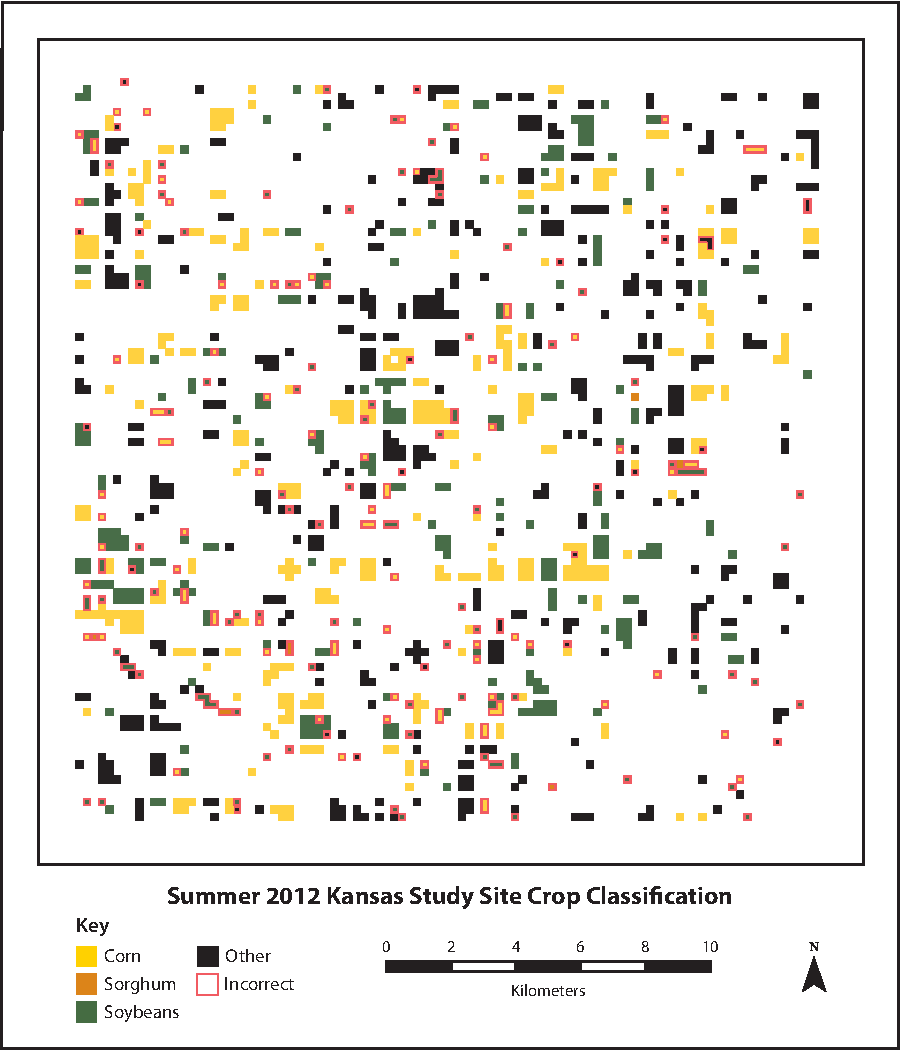
\includegraphics[width=\textwidth]{Graphics/KSclass.pdf}
  \caption[Kansas Summer 2012 Classification]{}
  \label{map:KSclassification}
\end{ssfigure}

\begin{sstable}
  \centering
  \caption{Summer 2012 Kansas Study Site Classification Accuracy}
  \label{table:ksresults}
  \begin{tabu}{rrrrrrrl}
    \toprule
    & & \multicolumn{4}{c}{\textbf{Reference Data}} & & \\
     &  & Corn & Soy & Sorghum & Other & Total & User Acc. \\
    \midrule
    \multirow{4}{*}{\rotatebox{90}{\textbf{Classified}}} & Corn & 369 & 65 & 5 & 17 & 456 & 80.92\% \\
     & Soy & 32 & 273 & 10 & 47 & 362 & 75.41\% \\
     & Sorghum & 0 & 0 & 2 & 6 & 8 & 25.00\% \\
     & Other & 13 & 16 & 1 & 503 & 533 & 94.37\% \\
     & Total & 414 & 354 & 18 & 573 & 1359 &  \\
     & Producer Acc.  & 89.13\% & 77.12\% & 11.11\% & 87.78\% &  &  \\
    \multicolumn{8}{r}{Overall Accuracy: 84.40\%} \\
    \multicolumn{8}{r}{Kappa: 0.76} \\
    \bottomrule
  \end{tabu}
\end{sstable}

\begin{table}[b]
  \begin{Spacing}{1.0}
  \centering
  \caption{Kansas Best Classification RMSE Thresholds}
  \label{table:ksbestthresh}
  \begin{tabu} to 4in {ZZ}
    \toprule
    \textbf{Signature} & \textbf{Threshold Value} \\
    \midrule
    Corn\_~1 & 1,000 \\
    Corn\_~2 & 750 \\
    Corn\_~3 & 500 \\
    Soy\_~1 & 750 \\
    Soy\_~2 & 1,300 \\
    Soy\_~3 & 500 \\
    Sorghum & 450 \\
    \bottomrule
  \end{tabu}
  \end{Spacing}
\end{table}

The Argentina classification had a top overall accuracy of 87.8 percent (\autoref{table:ARbestresult}). Looking more closely at the results, the accuracy seems to be skewed upward by the high number of non-summer-crop sample points, which were correctly classified as ``other.'' Within the summer crop sample points, the accuracy is much lower; only one of the twenty three soy points and zero of the two sorghum points were correctly classified. Corn fared a bit better, but was still underwhelming, as only 68.6 percent of the corn points were classified correctly. The RMSE thresholds used for this classification, in \autoref{table:ARbestthresh}, show that the Corn\_2 and Soy\_3 signatures contributed to the classification most heavily, the Corn\_1 and Soy\_2 signatures contributed only a little, and the Corn\_3, Soy\_1, and the Sorghum\_1 signatures did not contribute at all (hence the zero points of sorghum classified).

\begin{sstable}
  \centering
  \caption{Summer 2014 Pellegrini Best Classification Accuracy}
  \label{table:ARbestresult}
  \begin{tabu}{rrrrrrrl}
    \toprule
     & & \multicolumn{4}{c}{\textbf{Reference Data}} & & \\
     &  & Corn & Soy & Sorghum & Other & Total & User Acc. \\
    \midrule
    \multirow{4}{*}{\rotatebox{90}{\textbf{Classified}}} & Corn & 24 & 13 & 0 & 8 & 45 & 53.33\% \\
     & Soy & 0 & 2 & 1 & 2 & 5 & 40.00\% \\
     & Sorghum & 0 & 0 & 0 & 0 & 0 & 0.00\% \\
     & Other & 12 & 9 & 1 & 306 & 328 & 93.29\% \\
     & Total & 36 & 24 & 2 & 316 & 378 &  \\
     & Producer Acc. & 66.67\% & 8.33\% & 0.00\% & 96.84\% &  &  \\
    \multicolumn{8}{r}{Overall Accuracy: 87.83\%} \\
    \multicolumn{8}{r}{Kappa: 0.54} \\
    \bottomrule
  \end{tabu}
\end{sstable}

\begin{table}[b]
  \begin{Spacing}{1.0}
  \centering
  \caption{Pellegrini Best Classification RMSE Thresholds}
  \label{table:ARbestthresh}
  \begin{tabu} to 4in {ZZ}
    \toprule
    \textbf{Signature} & \textbf{Threshold Value} \\
    \midrule
    Corn\_1 & 550 \\
    Corn\_2 & 850 \\
    Corn\_3 & 0 \\
    Soy\_1 & 0 \\
    Soy\_2 & 600 \\
    Soy\_3 & 950 \\
    Sorghum\_1 & 0 \\
    \bottomrule
  \end{tabu}
  \end{Spacing}
\end{table}

A map of the classification, shown in \autoref{map:ARclassification}, illustrates how well the classification stayed within summer crop fields, and did not classify much beyond. However, almost all of the summer crop fields are classified as corn, reflecting the low summer crop accuracies shown in \autoref{table:ARbestresult}.

\begin{ssfigure}
  \centering
  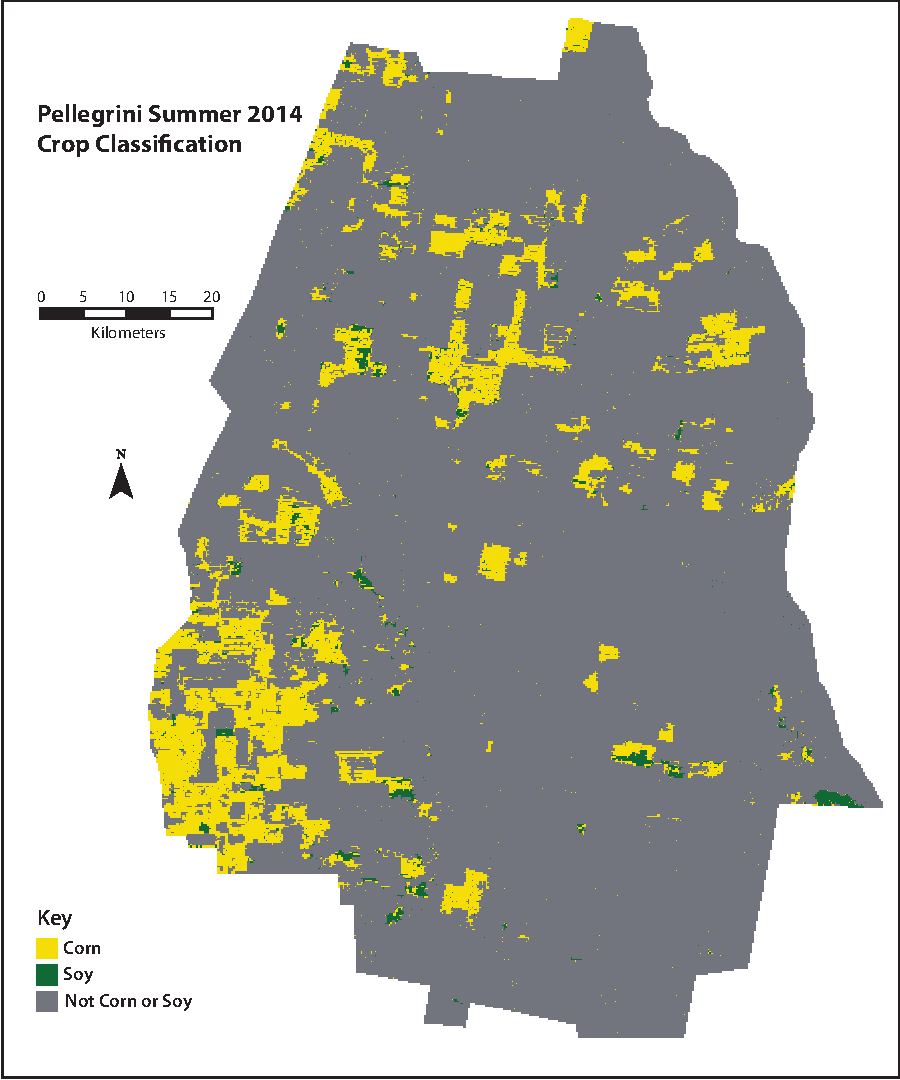
\includegraphics[width=\textwidth]{Graphics/ARclassed.pdf}
  \caption[Pellegrini Summer 2014 Classification]{}
  \label{map:ARclassification}
\end{ssfigure}